% The Lattice Phase System: First-Class Immutability with Dual-Heap Memory Management
%
% Compile with: pdflatex lattice_paper.tex && pdflatex lattice_paper.tex
%
\documentclass[11pt]{article}

\usepackage[margin=1in]{geometry}
\usepackage{amsmath,amssymb,amsthm}
\usepackage{mathpartir}
\usepackage{stmaryrd}        % \llbracket, \rrbracket
\usepackage{xcolor}
\usepackage{microtype}
\usepackage{enumitem}
\usepackage{booktabs}
\usepackage{multirow}
\usepackage{listings}
\usepackage{tikz}
\usepackage{pgfplots}
\usepackage{pgfplotstable}
\usepackage{hyperref}
\usepackage[title]{appendix}
\usepackage{float}

\usetikzlibrary{shapes.geometric, arrows.meta, positioning, fit, backgrounds, calc}
\pgfplotsset{compat=1.17}

% Lightning bolt for errors
\newcommand{\errormark}{\,\text{\textdagger}}

% ── Theorem environments ──
\newtheorem{theorem}{Theorem}[section]
\newtheorem{lemma}[theorem]{Lemma}
\newtheorem{proposition}[theorem]{Proposition}
\newtheorem{corollary}[theorem]{Corollary}
\newtheorem{definition}[theorem]{Definition}
\newtheorem{remark}[theorem]{Remark}

% ── Notation macros ──
\newcommand{\kw}[1]{\mathbf{#1}}
\newcommand{\flx}{\kw{flux}}
\newcommand{\fixkw}{\kw{fix}}
\newcommand{\letkw}{\kw{let}}
\newcommand{\freezekw}{\kw{freeze}}
\newcommand{\thawkw}{\kw{thaw}}
\newcommand{\clonekw}{\kw{clone}}
\newcommand{\forgekw}{\kw{forge}}
\newcommand{\returnkw}{\kw{return}}
\newcommand{\spawnkw}{\kw{spawn}}

% Phase tags
\newcommand{\fluid}{\mathsf{fluid}}
\newcommand{\crystal}{\mathsf{crystal}}
\newcommand{\unphased}{\bot}

% Phase set
\newcommand{\Phase}{\mathsf{Phase}}

% Semantic domains
\newcommand{\Val}{\mathsf{Val}}
\newcommand{\TVal}{\mathsf{TVal}}
\newcommand{\Env}{\mathsf{Env}}
\newcommand{\Store}{\mathsf{Store}}
\newcommand{\Loc}{\mathsf{Loc}}
\newcommand{\Region}{\mathsf{Region}}
\newcommand{\RegId}{\mathsf{RId}}
\newcommand{\FHeap}{\mathsf{FHeap}}
\newcommand{\RStore}{\mathsf{RStore}}
\newcommand{\Arena}{\mathsf{Arena}}
\newcommand{\Page}{\mathsf{Page}}
\newcommand{\Expr}{\mathsf{Expr}}
\newcommand{\Stmt}{\mathsf{Stmt}}
\newcommand{\Decl}{\mathsf{Decl}}
\newcommand{\Var}{\mathsf{Var}}

% Tagged value notation
\newcommand{\tval}[2]{#1^{#2}}

% Deep clone
\newcommand{\dc}[1]{\mathsf{deepclone}(#1)}

% Judgment forms
\newcommand{\phchk}[2]{#1 \vdash #2\ \mathbf{ok}}
\newcommand{\phexpr}[3]{#1 \vdash #2 : #3}

% Store operations
\newcommand{\dom}{\mathrm{dom}}
\newcommand{\migrate}{\rightsquigarrow}

% Evaluation
\newcommand{\bigeval}[5]{\langle #1, #2 \rangle \Downarrow_{#3} \langle #4, #5 \rangle}
\newcommand{\evstmt}[4]{\langle #1, #2 \rangle \Downarrow \langle #3, #4 \rangle}

% ── Listings configuration ──
\lstdefinelanguage{Lattice}{
  morekeywords={fn,let,flux,fix,struct,if,else,for,in,while,return,freeze,thaw,clone,forge,true,false,print,spawn},
  sensitive=true,
  morecomment=[l]{//},
  morecomment=[s]{/*}{*/},
  morestring=[b]",
  literate={->}{$\rightarrow$}{2},
}
\lstset{
  language=Lattice,
  basicstyle=\small\ttfamily,
  keywordstyle=\bfseries,
  commentstyle=\itshape\color{gray},
  stringstyle=\color{darkgray},
  numbers=left,
  numberstyle=\tiny\color{gray},
  numbersep=5pt,
  frame=single,
  framesep=3pt,
  xleftmargin=1.5em,
  breaklines=true,
  captionpos=b,
  aboveskip=0.8\baselineskip,
  belowskip=0.5\baselineskip,
}

% ── Document ──
\title{\textbf{The Lattice Phase System:\\First-Class Immutability with Dual-Heap Memory Management}}
\author{Alex Jokela\\{\small\texttt{alex.c.jokela@gmail.com}}}
\date{February 2026}

\begin{document}
\maketitle

\begin{abstract}
Dynamic languages typically treat mutability as the default and offer
immutability only as an advisory annotation (JavaScript's
\texttt{Object.freeze}) or through separate type hierarchies (Scala's
\texttt{val}/\texttt{var}).  We present \emph{Lattice}, a dynamically
typed language whose runtime associates every value with a \emph{phase
tag}---either $\fluid$ (mutable) or $\crystal$ (deeply immutable)---and
mediates all transitions through explicit $\freezekw$, $\thawkw$,
$\clonekw$, and $\forgekw$ operations.  The phase system is backed by a
\emph{dual-heap memory architecture}: a garbage-collected fluid heap for
mutable data and an arena-based region store for crystal (frozen) data,
connected by a freeze migration protocol that deep-clones values into
arena regions and establishes full pointer disjointness between heaps.

We formalize the phase system with a big-step operational semantics and
static phase-checking rules, and prove six key safety properties: phase
monotonicity, value isolation, consuming freeze semantics, forge
soundness, heap separation, and thaw independence.  Empirical evaluation
across eight benchmarks shows that the dual-heap architecture adds less
than 2\% wall-clock overhead compared to a single-heap baseline, with
RSS costs proportional to frozen data volume.  The architecture provides
a foundation for future optimizations including copy-on-write sharing,
concurrent collection, and safe parallelism via the crystal-implies-shareable
invariant.
\end{abstract}

%% ════════════════════════════════════════════════════════════════════
\section{Introduction}
\label{sec:intro}

Mutable state is a perennial source of bugs in dynamic languages.
Aliasing permits distant mutations to corrupt shared data structures;
defensive copying wastes memory and CPU cycles; and garbage collectors
must trace the entire heap regardless of whether values are long-lived
and unchanging.  Consider a game engine that periodically snapshots
its state for rollback:

\begin{figure}[t]
\begin{lstlisting}[caption={Game rollback in Lattice: mutable state is checkpointed by freezing and restored by thawing.},label=fig:game-rollback]
struct GameState {
    frame: Int, score: Int,
    player_x: Int, player_y: Int,
    hp: Int, entities: Array,
}

fn main() {
    let checkpoints = []
    let state = GameState {
        frame: 0, score: 0,
        player_x: 100, player_y: 100,
        hp: 100, entities: make_entities(20),
    }
    for f in 0..500 {
        state = tick(state)
        // Checkpoint every 25 frames
        if state.frame % 25 == 0 {
            let cp = freeze(clone(state))
            checkpoints.push(cp)
        }
        // Rollback on desync
        if state.frame % 100 == 0 {
            if checkpoints.len() > 1 {
                let idx = checkpoints.len() - 2
                state = thaw(checkpoints[idx])
            }
        }
    }
}
\end{lstlisting}
\end{figure}

In a conventional dynamic language, the programmer must manually ensure
that checkpoints are truly independent of the live state---a single
shared reference suffices to corrupt the snapshot.  JavaScript's
\texttt{Object.freeze} is shallow and advisory; Python has no built-in
mechanism; and even Clojure's persistent data structures require the
programmer to consistently use the functional API.

Lattice addresses this problem by making immutability a \emph{first-class
runtime property}.  Every value carries a phase tag---$\fluid$ for
mutable, $\crystal$ for deeply immutable---and the runtime enforces
phase discipline through explicit transition operations.  In
Figure~\ref{fig:game-rollback}, \texttt{freeze(clone(state))} produces
a crystal checkpoint: a deeply immutable, independently allocated
snapshot that the garbage collector can skip during mark traversal and
that can be bulk-deallocated when the checkpoint becomes unreachable.

\paragraph{Contributions.}
This paper makes three contributions:

\begin{enumerate}[nosep]
  \item \textbf{The Lattice phase system} (\S\ref{sec:overview}--\S\ref{sec:static}):
    a runtime discipline where every value is tagged $\fluid$ or
    $\crystal$, with explicit $\freezekw$/$\thawkw$/$\clonekw$/$\forgekw$
    operations mediating all phase transitions.  A static phase checker
    provides early error detection in strict mode.

  \item \textbf{A dual-heap memory architecture} (\S\ref{sec:implementation}):
    a garbage-collected fluid heap paired with an arena-based region
    store, connected by a freeze migration protocol that establishes
    full pointer disjointness.  We prove six safety properties
    (\S\ref{sec:properties}), including heap separation (no crystal
    pointer appears in the fluid allocation list) and phase monotonicity
    (crystal values cannot be mutated in place).  Full proofs appear in
    Appendix~\ref{app:proofs}.

  \item \textbf{Empirical validation} (\S\ref{sec:evaluation}):
    across eight benchmarks spanning allocation-heavy, closure-heavy,
    event-sourcing, and snapshot-based workloads, the dual-heap
    architecture adds less than 2\% wall-clock overhead to the two
    heaviest benchmarks (event sourcing at 1.0\,s and game rollback at
    1.9\,s), with RSS costs proportional to frozen data volume.
\end{enumerate}

%% ════════════════════════════════════════════════════════════════════
\section{Language Overview}
\label{sec:overview}

Lattice is a dynamically typed, expression-oriented language with
C-like syntax, first-class closures, structs, arrays, and maps.  Its
distinguishing feature is the \emph{phase system}: every runtime value
carries a phase tag that is either $\fluid$ (mutable) or $\crystal$
(deeply immutable).

\subsection{Declarations and Phase Tags}

Lattice provides three declaration keywords that determine the initial
phase of a binding:

\begin{itemize}[nosep]
  \item \texttt{flux x = e} --- declares $x$ with phase $\fluid$
    (mutable).  The value may be reassigned and its sub-values may be
    mutated in place.
  \item \texttt{fix x = e} --- declares $x$ with phase $\crystal$
    (immutable).  The initializer is automatically frozen and migrated
    to the region store.  Any attempt to reassign or mutate $x$ is
    rejected.
  \item \texttt{let x = e} --- infers the phase from the initializer
    (casual mode) or is rejected in strict mode, where the programmer
    must choose explicitly.
\end{itemize}

\noindent
A simple example:

\begin{lstlisting}[caption={Phase declarations and transitions.},label=fig:phase-decl]
#mode strict
flux counter = 0       // fluid: mutable
counter += 1           // OK
fix pi = freeze(3.14)  // crystal: immutable
// pi = 2.71           // ERROR: cannot assign to crystal
flux thawed = thaw(pi) // deep clone into fluid heap
thawed = 2.71          // OK: thawed is fluid
\end{lstlisting}

\subsection{Phase Transition Operations}

Four operations mediate phase transitions:

\begin{description}[nosep,labelwidth=1.5cm]
  \item[\texttt{freeze(e)}] Evaluates $e$, sets all phase tags to
    $\crystal$ recursively, deep-clones the value into an arena region,
    and frees the original fluid pointers.  In strict mode, freezing a
    variable \emph{consumes} the binding (use-after-freeze is an error).
  \item[\texttt{thaw(e)}] Deep-clones the value and sets all phase tags
    to $\fluid$.  The original crystal value is unaffected.
  \item[\texttt{clone(e)}] Deep-clones the value, preserving the
    original phase.  Useful for creating independent copies of mutable
    data.
  \item[\texttt{forge \{ ... \}}] A block expression that evaluates its
    body, then automatically freezes the result.  Forge blocks are
    \emph{compositional factories}: their output is guaranteed crystal.
\end{description}

\begin{figure}[t]
\centering
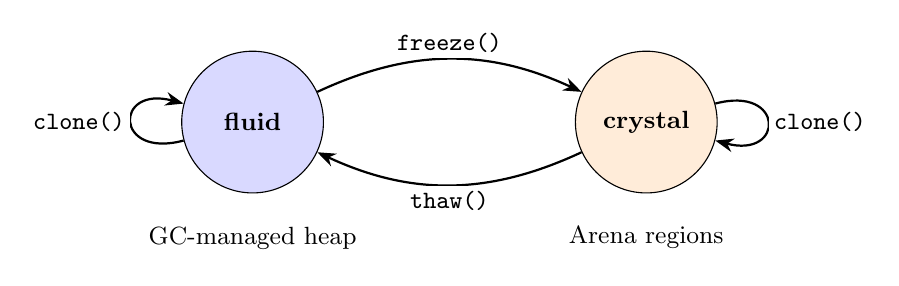
\begin{tikzpicture}[
  state/.style={circle, draw, minimum size=1.8cm, font=\small\bfseries},
  every edge/.style={draw, -Stealth, thick},
  label/.style={font=\small, fill=white, inner sep=2pt},
]
  \node[state, fill=blue!15] (fluid)   at (0,0)   {fluid};
  \node[state, fill=orange!15] (crystal) at (5,0)   {crystal};

  \draw (fluid) edge[bend left=25] node[label, above] {\texttt{freeze()}} (crystal);
  \draw (crystal) edge[bend left=25] node[label, below] {\texttt{thaw()}} (fluid);
  \draw (fluid) edge[loop left, looseness=5] node[label, left] {\texttt{clone()}} (fluid);
  \draw (crystal) edge[loop right, looseness=5] node[label, right] {\texttt{clone()}} (crystal);

  \node[font=\small, below=0.3cm] at (fluid.south) {GC-managed heap};
  \node[font=\small, below=0.3cm] at (crystal.south) {Arena regions};
\end{tikzpicture}
\caption{Phase transition state diagram.  \texttt{freeze} migrates values
from the fluid heap to arena regions; \texttt{thaw} deep-clones back.
\texttt{clone} produces independent copies within the same heap.}
\label{fig:phase-diagram}
\end{figure}

Figure~\ref{fig:phase-diagram} shows the state diagram.  The key
design principle is that \emph{all transitions are explicit and
deep}: freezing recursively freezes all sub-values, and thawing produces
a fully independent mutable copy.

\subsection{Strict Mode and Static Checking}

Lattice programs operate in one of two modes:
\begin{itemize}[nosep]
  \item \textbf{Casual mode} (default): \texttt{let} is permitted, phase
    violations produce warnings, and freeze updates bindings in place.
  \item \textbf{Strict mode} (\texttt{\#mode strict}): \texttt{let} is
    rejected (use \texttt{flux} or \texttt{fix}), crystal assignments are
    errors, and freeze \emph{consumes} the binding.
\end{itemize}

\noindent
Strict mode provides a lightweight form of affine resource management:
$\freezekw : \tau^{\fluid} \multimap \tau^{\crystal}$, where the linear
arrow $\multimap$ indicates that the fluid binding is consumed.  This
prevents use-after-freeze bugs without requiring a full linear type
system.

\subsection{Event Sourcing Example}

\begin{figure}[t]
\begin{lstlisting}[caption={Event sourcing: frozen events form an append-only log.},label=fig:event-sourcing]
struct Event { kind: String, amount: Int, seq: Int }
struct Account { balance: Int, tx_count: Int }

fn apply_event(acct: Account, evt: Event) -> Account {
    if evt.kind == "deposit" {
        return Account {
            balance: acct.balance + evt.amount,
            tx_count: acct.tx_count + 1
        }
    }
    if evt.kind == "withdraw" {
        return Account {
            balance: acct.balance - evt.amount,
            tx_count: acct.tx_count + 1
        }
    }
    return acct
}

fn replay(events: Array, count: Int) -> Account {
    let acct = Account { balance: 0, tx_count: 0 }
    for i in 0..count {
        let evt = thaw(events[i])
        acct = apply_event(acct, evt)
    }
    return acct
}

fn main() {
    let event_log = []
    for i in 0..200 {
        let kind = "deposit"
        if i % 3 == 0 { kind = "withdraw" }
        let evt = Event { kind: kind,
            amount: (i % 50) + 1, seq: i }
        event_log.push(freeze(evt))
    }
    // Replay at periodic intervals
    for checkpoint in 0..5 {
        let count = (checkpoint + 1) * 40
        let state = replay(event_log, count)
    }
}
\end{lstlisting}
\end{figure}

Figure~\ref{fig:event-sourcing} demonstrates an event-sourcing pattern.
Each event is frozen immediately upon creation, forming an append-only
log of crystal values.  State is rebuilt by thawing and replaying events.
The phase system guarantees that events are never accidentally mutated
after insertion into the log, and the dual-heap architecture ensures
that long-lived frozen events reside in arena regions that are
bulk-deallocated when the log is discarded.

\subsection{Forge Blocks}

Forge blocks provide a controlled-mutation pattern for constructing
immutable data:

\begin{lstlisting}[caption={Forge block for constructing immutable configuration.},label=fig:forge-example]
fix config = forge {
    flux temp = Map::new()
    temp.set("host", "localhost")
    temp.set("port", "8080")
    temp.set("debug", "true")
    freeze(temp)
}
// config is crystal --- mutations are rejected
\end{lstlisting}

\noindent
The body of a forge block may use arbitrary mutable operations; the
result is automatically frozen.  Forge blocks compose: nested forge
blocks each produce crystal output, and the outer forge's freeze on
an already-crystal value is idempotent.

%% ════════════════════════════════════════════════════════════════════
\section{Formal Semantics}
\label{sec:formal}

We present the formal semantics of the Lattice phase system, comprising
semantic domains, abstract syntax, static phase-checking rules,
big-step operational semantics, and the dual-heap memory model.

\subsection{Phase Tags and Semantic Domains}
\label{sec:domains}

\begin{definition}[Phase Tags]
The set of \emph{phase tags} is:
$\sigma \in \Phase \triangleq \{ \fluid,\; \crystal,\; \unphased \}$,
where $\fluid$ denotes mutable data, $\crystal$ denotes deeply immutable
data, and $\unphased$ ($\bot$) denotes data whose phase has not been
explicitly specified.
\end{definition}

\begin{definition}[Tagged Values]
A \emph{tagged value} is a pair $\tval{v}{\sigma}$ where $v$ is a raw value
and $\sigma \in \Phase$ is its phase tag.  The raw value domain is:
\[
  v \in \Val ::= n \mid r \mid b \mid s \mid [v_1, \ldots, v_k]
    \mid S\{f_1\!:\!v_1, \ldots, f_k\!:\!v_k\}
    \mid \langle \bar{x}, e, \rho \rangle
    \mid ()
    \mid \{s_1\!:\!v_1, \ldots, s_k\!:\!v_k\}
\]
where $n \in \mathbb{Z}$, $r \in \mathbb{R}$, $b \in \mathbb{B}$,
$s \in \mathsf{String}$, and $\langle \bar{x}, e, \rho \rangle$ is a
closure with parameters $\bar{x}$, body $e$, and captured environment
$\rho$.
\end{definition}

\begin{definition}[Environments and Stores]
An \emph{environment} $\rho : \Var \rightharpoonup \TVal$ maps variable
names to tagged values.  Variable lookup produces a \emph{deep clone}:
$\rho(x) = \dc{\rho_{\mathrm{raw}}(x)}$.
This ensures \emph{value isolation}: the caller receives an independent
copy.
\end{definition}

\begin{definition}[Dual-Heap Store]
\label{def:dual-heap}
The \emph{store} $\mu = (\mathcal{F}, \mathcal{R})$ is a disjoint union
of a \emph{fluid heap}
$\mathcal{F} \in \FHeap$ (tracked allocations managed by mark-sweep GC;
all $\fluid$- and $\unphased$-tagged values reside here) and a
\emph{region store} $\mathcal{R} \in \RStore = \RegId \rightharpoonup
\Region$ (arena-allocated regions; all $\crystal$-tagged values reside
in exactly one region).
\end{definition}

\subsection{Abstract Syntax}
\label{sec:syntax}

\[
\begin{array}{rcll}
  d \in \Decl &::=& \flx\; x = e
                    \mid \fixkw\; x = e
                    \mid \letkw\; x = e
              & \text{(declarations)} \\[4pt]
  e \in \Expr &::=& x \mid c \mid e_1 \oplus e_2
                    \mid [e_1, \ldots, e_k]
                    \mid S\{f_1\!:\!e_1, \ldots\}
              & \text{(base expressions)} \\
              &\mid& |x_1, \ldots, x_k|\; \{\ \bar{s}\ \}
              & \text{(closures)} \\
              &\mid& e.f \mid e[e'] \mid e(e_1, \ldots, e_k)
              & \text{(access, index, call)} \\
              &\mid& \freezekw(e) \mid \thawkw(e) \mid \clonekw(e)
              & \text{(phase operations)} \\
              &\mid& \forgekw\;\{\ \bar{s}\ \}
              & \text{(forge block)} \\[4pt]
  s \in \Stmt &::=& d \mid x = e \mid e \mid \returnkw\; e
              & \text{(statements)} \\
              &\mid& \kw{for}\; x\; \kw{in}\; e\; \{\ \bar{s}\ \}
                    \mid \kw{while}\; e\; \{\ \bar{s}\ \}
              & \text{(loops)} \\
\end{array}
\]
Programs operate in mode $\mathcal{M} \in \{ \mathsf{casual}, \mathsf{strict} \}$.

\subsection{Static Phase Checking}
\label{sec:static}

The static phase checker maintains a context
$\Gamma : \Var \rightharpoonup \Phase$ and infers phases for expressions
via $\phexpr{\Gamma}{e}{\sigma}$ (``under $\Gamma$, expression $e$ has
phase $\sigma$'').

\begin{figure}[t]
\begin{mathpar}
  \inferrule*[lab=\textsc{PC-Freeze}]
    {\phexpr{\Gamma}{e}{\sigma} \\
     \mathcal{M} = \mathsf{strict} \Rightarrow \sigma \neq \crystal}
    {\phexpr{\Gamma}{\freezekw(e)}{\crystal}}

  \inferrule*[lab=\textsc{PC-Assign}]
    {\phexpr{\Gamma}{e}{\sigma_e} \\
     \mathcal{M} = \mathsf{strict} \Rightarrow \Gamma(x) \neq \crystal}
    {\phchk{\Gamma}{x = e}}

  \inferrule*[lab=\textsc{PC-Flux}]
    {\phexpr{\Gamma}{e}{\sigma_e} \\
     \mathcal{M} = \mathsf{strict} \Rightarrow \sigma_e \neq \crystal}
    {\phchk{\Gamma}{\flx\; x = e} \\
     \Gamma' = \Gamma[x \mapsto \fluid]}

  \inferrule*[lab=\textsc{PC-Fix}]
    {\phexpr{\Gamma}{e}{\sigma_e}}
    {\phchk{\Gamma}{\fixkw\; x = e} \\
     \Gamma' = \Gamma[x \mapsto \crystal]}

  \inferrule*[lab=\textsc{PC-Thaw}]
    {\phexpr{\Gamma}{e}{\sigma} \\
     \mathcal{M} = \mathsf{strict} \Rightarrow \sigma \neq \fluid}
    {\phexpr{\Gamma}{\thawkw(e)}{\fluid}}

  \inferrule*[lab=\textsc{PC-Forge}]
    {\Gamma' = \Gamma \\
     \forall s_i \in \bar{s}.\; \Gamma' \vdash s_i\ \mathbf{ok}}
    {\phexpr{\Gamma}{\forgekw\;\{\ \bar{s}\ \}}{\crystal}}

  \inferrule*[lab=\textsc{PC-Spawn-Strict}]
    {\mathcal{M} = \mathsf{strict} \\
     x \in \mathrm{FV}(\bar{s}) \\
     \Gamma(x) = \fluid}
    {\phchk{\Gamma}{\spawnkw\;\{\ \bar{s}\ \}}\errormark}
\end{mathpar}
\caption{Selected static phase-checking rules.  \textsc{PC-Freeze} ensures
already-crystal values are not double-frozen in strict mode.
\textsc{PC-Assign} prevents mutation of crystal bindings.
\textsc{PC-Flux} prevents aliasing crystal data as fluid.
\textsc{PC-Spawn-Strict} prevents fluid data from crossing thread
boundaries.}
\label{fig:static-rules}
\end{figure}

Figure~\ref{fig:static-rules} shows the key rules.  The
\textsc{PC-Spawn-Strict} rule is particularly noteworthy: it prevents
fluid (mutable) bindings from being captured across thread boundaries,
enforcing that shared data must be crystal.  This provides a foundation
for safe parallelism.

\subsection{Operational Semantics}
\label{sec:operational}

We define a big-step semantics with store-passing.  Configurations have
the form $\langle \rho, \mu, e \rangle$ and evaluate to
$\langle \mu', \tval{v}{\sigma} \rangle$.

\subsubsection{Variables and Literals}

\begin{mathpar}
  \inferrule*[lab=\textsc{E-Lit}]
    {c \text{ is a literal}}
    {\langle \rho, \mu, c \rangle \Downarrow
     \langle \mu, \tval{c}{\unphased} \rangle}

  \inferrule*[lab=\textsc{E-Var}]
    {\rho_{\mathrm{raw}}(x) = \tval{v}{\sigma} \\
     \tval{v'}{\sigma} = \dc{\tval{v}{\sigma}}}
    {\langle \rho, \mu, x \rangle \Downarrow
     \langle \mu, \tval{v'}{\sigma} \rangle}
\end{mathpar}

\noindent
\textsc{E-Var} deep-clones the stored value, ensuring value isolation:
every variable read yields an independent copy.

\subsubsection{Phase Transitions}

\begin{figure}[t]
\begin{mathpar}
  \inferrule*[lab=\textsc{E-Freeze-Strict}]
    {\mathcal{M} = \mathsf{strict} \\
     \rho_{\mathrm{raw}}(x) = \tval{v}{\sigma} \\
     \tval{v'}{\crystal} = \mathsf{setphase}(\tval{v}{\sigma}, \crystal) \\
     (\tval{v''}{\crystal}, \mathcal{R}') = \mathsf{freeze\_region}(\tval{v'}{\crystal}, \mathcal{R})}
    {\langle \rho, (\mathcal{F}, \mathcal{R}), \freezekw(x) \rangle \Downarrow
     \langle \rho \setminus x, (\mathcal{F}, \mathcal{R}'), \tval{v''}{\crystal} \rangle}

  \inferrule*[lab=\textsc{E-Freeze-Casual}]
    {\mathcal{M} = \mathsf{casual} \\
     \rho_{\mathrm{raw}}(x) = \tval{v}{\sigma} \\
     \tval{v'}{\crystal} = \mathsf{setphase}(\tval{v}{\sigma}, \crystal) \\
     (\tval{v''}{\crystal}, \mathcal{R}') = \mathsf{freeze\_region}(\tval{v'}{\crystal}, \mathcal{R}) \\
     \rho' = \rho[x \mapsto \tval{v''}{\crystal}]}
    {\langle \rho, (\mathcal{F}, \mathcal{R}), \freezekw(x) \rangle \Downarrow
     \langle \rho', (\mathcal{F}, \mathcal{R}'), \dc{\tval{v''}{\crystal}} \rangle}
\end{mathpar}
\caption{Freeze semantics.  In strict mode (\textsc{E-Freeze-Strict}),
the binding is \emph{consumed}: $\rho \setminus x$ removes $x$ from the
environment.  In casual mode (\textsc{E-Freeze-Casual}), the binding is
updated in place.  Both modes migrate the value to an arena region.}
\label{fig:freeze-rules}
\end{figure}

Figure~\ref{fig:freeze-rules} contrasts strict and casual freeze.  The
critical difference is that strict-mode freeze removes the binding
($\rho \setminus x$), preventing use-after-freeze.

Thaw deep-clones a value and sets its phase to $\fluid$:
\begin{mathpar}
  \inferrule*[lab=\textsc{E-Thaw-Var}]
    {\rho_{\mathrm{raw}}(x) = \tval{v}{\sigma} \\
     \tval{v'}{\fluid} = \dc{\tval{v}{\sigma}}[\sigma := \fluid] \\
     \rho' = \rho[x \mapsto \tval{v'}{\fluid}]}
    {\langle \rho, \mu, \thawkw(x) \rangle \Downarrow
     \langle \rho', \mu, \dc{\tval{v'}{\fluid}} \rangle}
\end{mathpar}

Clone preserves the original phase:
\begin{mathpar}
  \inferrule*[lab=\textsc{E-Clone}]
    {\langle \rho, \mu, e \rangle \Downarrow
     \langle \mu', \tval{v}{\sigma} \rangle \\
     \tval{v'}{\sigma} = \dc{\tval{v}{\sigma}}}
    {\langle \rho, \mu, \clonekw(e) \rangle \Downarrow
     \langle \mu', \tval{v'}{\sigma} \rangle}
\end{mathpar}

Forge evaluates its body and freezes the result:
\begin{mathpar}
  \inferrule*[lab=\textsc{E-Forge}]
    {\langle \rho', \mu, \bar{s} \rangle \Downarrow_{\mathit{block}}
     \langle \mu', \tval{v}{\sigma} \rangle \\
     \tval{v'}{\crystal} = \mathsf{setphase}(\tval{v}{\sigma}, \crystal) \\
     (\tval{v''}{\crystal}, \mathcal{R}') = \mathsf{freeze\_region}(\tval{v'}{\crystal}, \mathcal{R}')}
    {\langle \rho, \mu, \forgekw\;\{\ \bar{s}\ \} \rangle \Downarrow
     \langle (\mathcal{F}', \mathcal{R}'), \tval{v''}{\crystal} \rangle}
\end{mathpar}

\subsubsection{Binding Declarations}

\begin{mathpar}
  \inferrule*[lab=\textsc{E-Flux}]
    {\langle \rho, \mu, e \rangle \Downarrow
     \langle \mu', \tval{v}{\sigma} \rangle \\
     \mathcal{M} = \mathsf{strict} \Rightarrow \sigma \neq \crystal}
    {\langle \rho, \mu, \flx\; x = e \rangle \Downarrow
     \langle \rho[x \mapsto \tval{v}{\fluid}], \mu', () \rangle}

  \inferrule*[lab=\textsc{E-Fix}]
    {\langle \rho, \mu, e \rangle \Downarrow
     \langle \mu', \tval{v}{\sigma} \rangle \\
     \tval{v'}{\crystal} = \mathsf{setphase}(\tval{v}{\sigma}, \crystal) \\
     (\tval{v''}{\crystal}, \mathcal{R}') = \mathsf{freeze\_region}(\tval{v'}{\crystal}, \mathcal{R}')}
    {\langle \rho, \mu, \fixkw\; x = e \rangle \Downarrow
     \langle \rho[x \mapsto \tval{v''}{\crystal}], (\mathcal{F}', \mathcal{R}'), () \rangle}
\end{mathpar}

\subsubsection{Assignment and Lvalue Resolution}

Assignment uses \emph{lvalue resolution} to obtain a mutable pointer
into the environment:
\begin{mathpar}
  \inferrule*[lab=\textsc{E-Assign}]
    {\langle \rho, \mu, e \rangle \Downarrow
     \langle \mu', \tval{v}{\sigma} \rangle \\
     \rho_{\mathrm{raw}}(x) = \tval{v_0}{\sigma_0} \\
     \mathcal{M} = \mathsf{strict} \Rightarrow \sigma_0 \neq \crystal}
    {\langle \rho, \mu, x = e \rangle \Downarrow
     \langle \rho[x \mapsto \tval{v}{\sigma}], \mu', () \rangle}

  \inferrule*[lab=\textsc{E-Assign-Crystal-Err}]
    {\mathcal{M} = \mathsf{strict} \\
     \rho_{\mathrm{raw}}(x) = \tval{v_0}{\crystal}}
    {\langle \rho, \mu, x = e \rangle \Downarrow
     \mathsf{error}(\text{``cannot assign to crystal binding''})}
\end{mathpar}

\noindent
The read/write asymmetry is a defining characteristic: \emph{reads}
always deep-clone (via \textsc{E-Var}), ensuring value isolation, while
\emph{writes} resolve lvalue paths to direct pointers, enabling
efficient in-place mutation of fluid data.

\subsection{Memory Model}
\label{sec:memory-model}

\subsubsection{Fluid Heap}

The fluid heap $\mathcal{F} = \{ (p_i, n_i, m_i) \}_{i \in I}$ is a
set of tracked allocations where $p_i$ is a pointer, $n_i$ is the
allocation size, and $m_i \in \{0, 1\}$ is the GC mark bit.  The
garbage collector uses a three-phase mark-sweep protocol:
(1)~\emph{unmark} all allocations;
(2)~\emph{mark} all reachable values from root environments, saved
caller environments, and the shadow stack---for crystal values with a
valid region ID, record the region ID and return immediately;
(3)~\emph{sweep} unmarked fluid allocations and collect unreachable
regions.

\subsubsection{Region Store and Arena Allocation}

\begin{definition}[Crystal Region]
A crystal region $R = (r, \varepsilon, P, n)$ consists of a unique
identifier $r \in \RegId$, an epoch $\varepsilon$, a linked list of
arena pages $P$ (each 4096 bytes), and total bytes used $n$.
Arena allocation is $O(1)$ amortized (bump-pointer within a page).
\end{definition}

\begin{definition}[Region Collection]
Given reachable region IDs $\mathcal{S} \subseteq \RegId$ from the mark
phase:
$\mathsf{region\_collect}(\mathcal{R}, \mathcal{S}) =
\{ r \mapsto R \mid (r \mapsto R) \in \mathcal{R},\; r \in \mathcal{S} \}$.
Unreachable regions are freed in $O(|P|)$ time per region---bulk
deallocation without per-object overhead.
\end{definition}

\subsubsection{Freeze Migration Protocol}

The central operation linking the two heaps is
$\mathsf{freeze\_region}(\tval{v}{\crystal}, (\mathcal{F}, \mathcal{R}))$:
\begin{enumerate}[nosep]
  \item Create a fresh region $R$ with identifier $r$.
  \item Set the global arena pointer to $R$.
  \item Deep-clone $v$ into $R$: all allocations route through
    $\mathsf{arena\_alloc}(R, \cdot)$.
  \item Reset the arena pointer to null.
  \item Set $\mathsf{region\_id} := r$ on $v'$ and all sub-values.
  \item Free the original fluid-heap pointers.
  \item Return $\tval{v'}{\crystal}$ with updated $\mathcal{R}$.
\end{enumerate}

\noindent
After migration, the crystal value has completely independent pointers
from $\mathcal{F}$.

%% ════════════════════════════════════════════════════════════════════
\section{Properties and Proof Sketches}
\label{sec:properties}

We state six key safety properties.  Full proofs appear in
Appendix~\ref{app:proofs}.

\begin{table}[t]
\centering
\small
\renewcommand{\arraystretch}{1.3}
\begin{tabular}{@{}lp{9.5cm}@{}}
\toprule
\textbf{Theorem} & \textbf{Statement (informal)} \\
\midrule
Phase Monotonicity &
  Crystal values cannot be mutated in place: all assignment paths
  and mutating methods are blocked by runtime guards (strict mode) and
  static analysis. \\
Value Isolation &
  Variable reads produce independent copies: the returned value
  shares no mutable state with the environment's stored copy. \\
Consuming Freeze &
  In strict mode, freezing a variable removes it from the environment,
  preventing use-after-freeze. \\
Forge Soundness &
  The result of a forge block is always crystal-phased, regardless of
  the body's internal mutations. \\
Heap Separation &
  No pointer reachable from a crystal value with a valid region ID
  appears in the fluid heap's allocation list. \\
Thaw Independence &
  Thawing produces a fresh copy that shares no state with the source;
  the original crystal region is unaffected. \\
\bottomrule
\end{tabular}
\caption{The six safety properties of the Lattice phase system.}
\label{tbl:theorems}
\end{table}

Table~\ref{tbl:theorems} summarizes the six theorems.  We now state
each formally and provide proof sketches.

\begin{theorem}[Phase Monotonicity]
\label{thm:monotonicity}
If\/ $\tval{v}{\crystal}$ is a crystal-tagged value bound to variable
$x$, then for any assignment targeting $x$ or a sub-path of $x$,
evaluation in strict mode produces $\mathsf{error}$.
\end{theorem}

\begin{proof}[Proof sketch]
By exhaustive case analysis on all mutation paths: (I)~direct
assignment is blocked by \textsc{E-Assign-Crystal-Err}; (II)~compound
lvalue assignment is blocked by the post-resolution crystal guard,
which holds by induction on path length using the recursive phase
invariant of $\mathsf{setphase}$; (III)~mutating methods check
crystal phase on the receiver; (IV)~the static rule \textsc{PC-Assign}
rejects crystal assignments at analysis time.
See Appendix~\ref{app:proof-monotonicity}.
\end{proof}

\begin{theorem}[Value Isolation]
\label{thm:isolation}
If $\langle \rho, \mu, x \rangle \Downarrow \langle \mu,
\tval{v'}{\sigma} \rangle$, then $v'$ shares no mutable state with
$\rho_{\mathrm{raw}}(x)$:
$\mathsf{mreach}(\tval{v'}{\sigma}) \cap \mathsf{mreach}(\tval{v}{\sigma}) = \emptyset$.
\end{theorem}

\begin{proof}[Proof sketch]
By the \textsc{E-Var} rule, $v' = \dc{v}$.  The Deep Clone
Independence Lemma shows that $\mathsf{ptrs}(v') \cap \mathsf{ptrs}(v)
\subseteq \mathsf{arena}(\mathcal{R})$ by structural induction on
value types.  Any shared arena addresses are excluded from mutable
reachability by Phase Monotonicity.
See Appendix~\ref{app:proof-isolation}.
\end{proof}

\begin{theorem}[Consuming Freeze]
\label{thm:consuming}
In strict mode, after evaluating $\freezekw(x)$:
$x \notin \dom(\rho')$.
\end{theorem}

\begin{proof}[Proof sketch]
Direct from the \textsc{E-Freeze-Strict} rule: the resulting
environment is $\rho' = \rho \setminus x$, and by definition of
environment removal, $x \notin \dom(\rho')$.  Subsequent access to $x$
fails because \textsc{E-Var} requires $x \in \dom(\rho')$.
See Appendix~\ref{app:proof-consuming}.
\end{proof}

\begin{theorem}[Forge Soundness]
\label{thm:forge}
$\langle \rho, \mu, \forgekw\;\{\ \bar{s}\ \} \rangle \Downarrow
\langle \mu', \tval{v}{\sigma} \rangle \Longrightarrow \sigma = \crystal$.
\end{theorem}

\begin{proof}[Proof sketch]
By \textsc{E-Forge}, the body's result undergoes $\mathsf{setphase}$
(which is total and forces $\crystal$ by the Setphase Totality Lemma)
followed by $\mathsf{freeze\_region}$ (which preserves $\crystal$).
Error and signal cases hold vacuously.
See Appendix~\ref{app:proof-forge}.
\end{proof}

\begin{theorem}[Heap Separation]
\label{thm:separation}
$\forall\, \tval{v}{\crystal}$ with region $r$:
$\forall\, a \in \mathsf{ptrs}(v)$: $a \notin \dom(\mathcal{F})$.
\end{theorem}

\begin{proof}[Proof sketch]
By induction on the seven steps of the freeze migration protocol.
Arena pages are allocated via direct \texttt{malloc}, bypassing
$\mathsf{fluid\_alloc}$; the Arena Routing Completeness Lemma shows
all allocations during clone go to the arena; the Arena--Fluid
Disjointness Lemma shows no arena address appears in $\mathcal{F}$.
The original fluid pointers are freed in step~6.
See Appendix~\ref{app:proof-separation}.
\end{proof}

\begin{theorem}[Thaw Independence]
\label{thm:thaw}
$\langle \rho, \mu, \thawkw(e) \rangle \Downarrow \langle \mu',
\tval{v'}{\fluid} \rangle \Longrightarrow \mathsf{ptrs}(v') \cap
\mathsf{ptrs}(\llbracket e \rrbracket) = \emptyset$.
\end{theorem}

\begin{proof}[Proof sketch]
Since no freeze is in progress, $\mathsf{g\_arena} = \mathsf{null}$,
so all allocations in the deep clone go to the fluid heap.  Fresh
pointers are guaranteed disjoint from the source by the allocator
contract.  $\mathsf{setphase}$ modifies only phase tags, not pointers.
See Appendix~\ref{app:proof-thaw}.
\end{proof}

%% ════════════════════════════════════════════════════════════════════
\section{Implementation}
\label{sec:implementation}

Lattice is implemented in approximately 8,000 lines of C, comprising a
hand-written recursive-descent parser, a tree-walking evaluator, and
the dual-heap memory subsystem.  We describe the key implementation
decisions.

\subsection{Dual-Heap Architecture}

\begin{figure}[t]
\centering
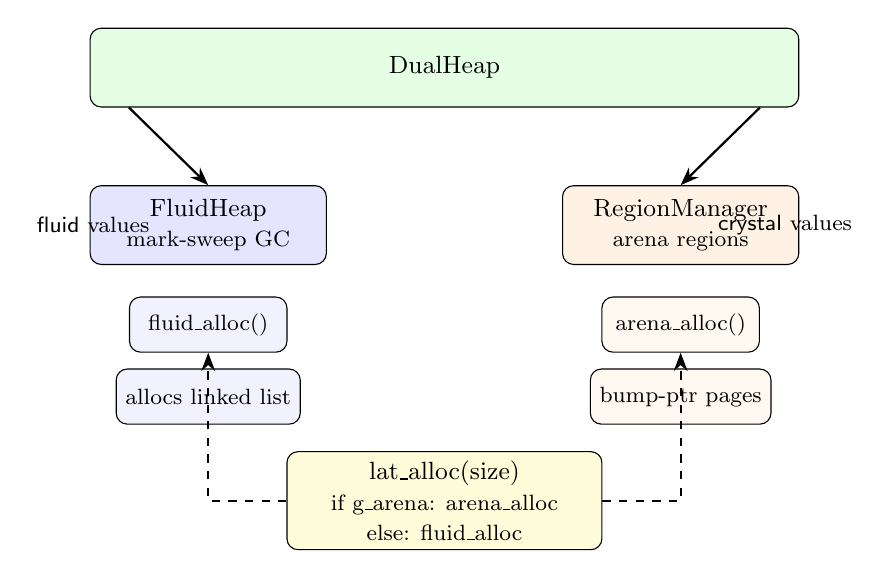
\begin{tikzpicture}[
  box/.style={draw, rounded corners, minimum width=3cm, minimum height=1cm,
              align=center, font=\small},
  smallbox/.style={draw, rounded corners, minimum width=2cm, minimum height=0.7cm,
                   align=center, font=\footnotesize},
  arr/.style={-Stealth, thick},
]
  % FluidHeap
  \node[box, fill=blue!10] (fluid) at (0, 0) {FluidHeap\\{\footnotesize mark-sweep GC}};
  \node[smallbox, fill=blue!5, below=0.4cm of fluid] (falloc) {fluid\_alloc()};
  \node[smallbox, fill=blue!5, below=0.2cm of falloc] (flist) {allocs linked list};

  % RegionManager
  \node[box, fill=orange!10] (regions) at (6, 0) {RegionManager\\{\footnotesize arena regions}};
  \node[smallbox, fill=orange!5, below=0.4cm of regions] (aalloc) {arena\_alloc()};
  \node[smallbox, fill=orange!5, below=0.2cm of aalloc] (pages) {bump-ptr pages};

  % DualHeap
  \node[box, fill=green!10, minimum width=9cm] (dual) at (3, 2)
       {DualHeap};

  % lat_alloc router
  \node[box, fill=yellow!15, minimum width=4cm] (router) at (3, -3.5)
       {lat\_alloc(size)\\{\footnotesize if g\_arena: arena\_alloc}\\
        {\footnotesize else: fluid\_alloc}};

  % Connections
  \draw[arr] (dual.south west) ++(0.5,0) -- (fluid.north);
  \draw[arr] (dual.south east) ++(-0.5,0) -- (regions.north);
  \draw[arr, dashed] (router) -| (falloc);
  \draw[arr, dashed] (router) -| (aalloc);

  % Labels
  \node[font=\footnotesize, anchor=west] at (-2.3, 0) {$\fluid$ values};
  \node[font=\footnotesize, anchor=east] at (8.3, 0) {$\crystal$ values};
\end{tikzpicture}
\caption{Dual-heap architecture.  The \texttt{lat\_alloc} router
directs allocations to the arena during freeze migration and to the
fluid heap otherwise.  The two heaps have disjoint address spaces.}
\label{fig:architecture}
\end{figure}

Figure~\ref{fig:architecture} shows the architecture.  The
\texttt{DualHeap} structure contains a \texttt{FluidHeap} (linked list
of tracked allocations with mark bits) and a \texttt{RegionManager}
(dynamic array of \texttt{CrystalRegion} pointers).

\subsection{Global Arena Routing}

The key implementation technique is a \emph{global arena pointer}
(\texttt{g\_arena}).  All value allocation functions---\texttt{lat\_alloc},
\texttt{lat\_calloc}, \texttt{lat\_strdup}---check this pointer first:

\begin{lstlisting}[language=C, basicstyle=\small\ttfamily,
  morekeywords={static,void,size_t,if,return,NULL},
  caption={Arena routing in \texttt{value.c}.},label=fig:arena-routing]
static CrystalRegion *g_arena = NULL;

static void *lat_alloc(size_t size) {
    if (g_arena) return arena_alloc(g_arena, size);
    if (g_heap)  return fluid_alloc(g_heap->fluid, size);
    return malloc(size);
}
\end{lstlisting}

\noindent
During \texttt{freeze\_to\_region}, the arena pointer is set before
deep-cloning and reset after, ensuring that \emph{every} allocation
in the clone---including strings, arrays, struct fields, map entries,
and closure environments---goes into the arena.  This is what
establishes the heap separation invariant (Theorem~\ref{thm:separation}).

\subsection{Garbage Collection with Crystal Fast-Path}

The GC mark phase traverses all reachable values.  When it encounters a
crystal value with a valid region ID, it records the region ID in a
reachable set and \emph{returns immediately}, without following any
pointers:

\begin{lstlisting}[language=C, basicstyle=\small\ttfamily,
  morekeywords={static,void,if,return,size_t},
  caption={Crystal fast-path in \texttt{gc\_mark\_value}.},label=fig:gc-crystal]
static void gc_mark_value(FluidHeap *fh, LatValue *v,
                          LatVec *reachable_regions) {
    if (v->phase == VTAG_CRYSTAL
        && v->region_id != (size_t)-1) {
        lat_vec_push(reachable_regions, &v->region_id);
        return;  // skip: all ptrs are in arena
    }
    // ... mark fluid pointers recursively
}
\end{lstlisting}

\noindent
This fast-path is safe because heap separation guarantees no crystal
pointer appears in the fluid allocation list.  The fast-path also
reduces GC pause time proportionally to the fraction of the object
graph that is crystal.

\subsection{Freeze Walkthrough}

The complete \texttt{freeze\_to\_region} function is 15 lines of C:

\begin{lstlisting}[language=C, basicstyle=\small\ttfamily,
  morekeywords={static,void,if,return,NULL},
  caption={The freeze migration protocol in \texttt{eval.c}.},label=fig:freeze-impl]
static void freeze_to_region(Evaluator *ev, LatValue *v) {
    if (ev->no_regions) return;
    CrystalRegion *region = region_create(
        ev->heap->regions);       // step 1
    value_set_arena(region);      // step 2
    LatValue clone = value_deep_clone(v); // step 3
    value_set_arena(NULL);        // step 4
    set_region_id_recursive(&clone, region->id); // step 5
    value_free(v);                // step 6
    *v = clone;                   // step 7
}
\end{lstlisting}

\noindent
The \texttt{no\_regions} flag enables a single-heap mode
(\texttt{-{}-no-regions}) used as the baseline in our evaluation.
In debug builds, \texttt{assert\_crystal\_not\_fluid} validates the
heap separation invariant after every GC cycle.

\begin{figure}[t]
\centering
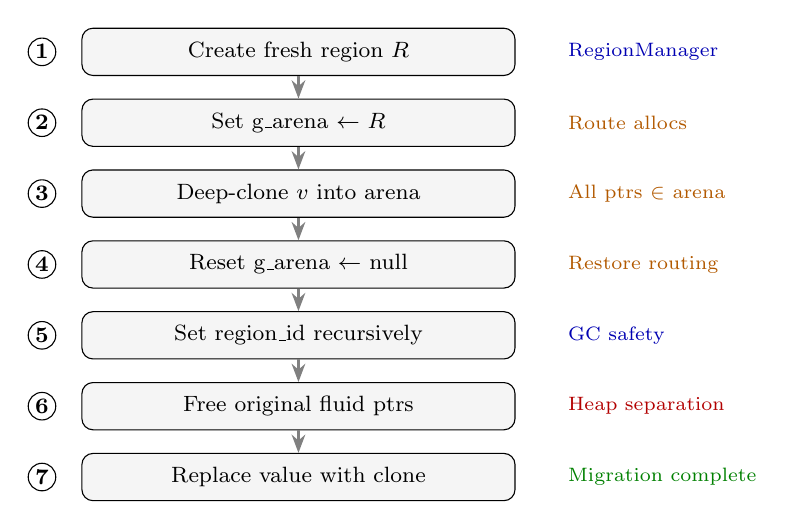
\begin{tikzpicture}[
  protostep/.style={draw, rounded corners, minimum width=5.5cm, minimum height=0.6cm,
               align=center, font=\footnotesize, fill=gray!8},
  arr/.style={-Stealth, thick, gray},
  num/.style={font=\footnotesize\bfseries, fill=white, circle, draw, inner sep=1pt},
]
  \node[protostep] (s1) at (0, 0)    {Create fresh region $R$};
  \node[protostep] (s2) at (0, -0.9) {Set g\_arena $\leftarrow$ $R$};
  \node[protostep] (s3) at (0, -1.8) {Deep-clone $v$ into arena};
  \node[protostep] (s4) at (0, -2.7) {Reset g\_arena $\leftarrow$ null};
  \node[protostep] (s5) at (0, -3.6) {Set region\_id recursively};
  \node[protostep] (s6) at (0, -4.5) {Free original fluid ptrs};
  \node[protostep] (s7) at (0, -5.4) {Replace value with clone};

  \foreach \i/\n in {s1/1,s2/2,s3/3,s4/4,s5/5,s6/6,s7/7} {
    \node[num] at ($(\i.west) + (-0.5,0)$) {\n};
  }
  \foreach \i/\j in {s1/s2,s2/s3,s3/s4,s4/s5,s5/s6,s6/s7} {
    \draw[arr] (\i) -- (\j);
  }

  % Side annotations
  \node[font=\scriptsize, anchor=west, text=blue!70!black] at (3.3, 0) {RegionManager};
  \node[font=\scriptsize, anchor=west, text=orange!70!black] at (3.3, -0.9) {Route allocs};
  \node[font=\scriptsize, anchor=west, text=orange!70!black] at (3.3, -1.8) {All ptrs $\in$ arena};
  \node[font=\scriptsize, anchor=west, text=orange!70!black] at (3.3, -2.7) {Restore routing};
  \node[font=\scriptsize, anchor=west, text=blue!70!black] at (3.3, -3.6) {GC safety};
  \node[font=\scriptsize, anchor=west, text=red!70!black] at (3.3, -4.5) {Heap separation};
  \node[font=\scriptsize, anchor=west, text=green!50!black] at (3.3, -5.4) {Migration complete};
\end{tikzpicture}
\caption{The seven-step freeze migration protocol.  Steps 2--4
bracket the deep-clone operation, ensuring all allocations route
through the arena.  Step 6 removes original pointers from the fluid
heap, completing heap separation.}
\label{fig:freeze-protocol}
\end{figure}

%% ════════════════════════════════════════════════════════════════════
\section{Evaluation}
\label{sec:evaluation}

We evaluate the dual-heap architecture empirically, comparing the
full region-based implementation against a single-heap baseline
(\texttt{-{}-no-regions}) that retains the phase system but skips
arena migration.

\subsection{Experimental Setup}

\paragraph{Platform.}
All experiments run on macOS (Darwin 25.2.0) with Apple Silicon.  The
Lattice interpreter is compiled with \texttt{clang -O2}.

\paragraph{Methodology.}
Each benchmark runs 20 times per mode (regions vs.\ no-regions).  We
report mean wall-clock time with standard deviation, and peak RSS from
the interpreter's internal memory statistics.  The \texttt{-{}-no-regions}
flag disables arena allocation: \texttt{freeze} sets the phase tag but
does not create a region or deep-clone into arena pages.  This isolates
the cost of the dual-heap mechanism itself.

\subsection{Benchmark Suite}

\begin{table}[t]
\centering
\small
\renewcommand{\arraystretch}{1.2}
\begin{tabular}{@{}llrr@{}}
\toprule
\textbf{Benchmark} & \textbf{Description} & \textbf{Freezes} & \textbf{Thaws} \\
\midrule
alloc\_churn      & GC stress: tight alloc/drop loop        & 0     & 0     \\
closure\_heavy    & Nested map/filter chains                 & 0     & 0     \\
event\_sourcing   & Frozen event log with periodic replay    & 200   & 600   \\
freeze\_thaw\_cycle & Rapid freeze/thaw of structs           & 1,000 & 1,000 \\
game\_rollback    & Periodic checkpoints with rollback       & 20    & 5     \\
long\_lived\_crystal & Long-lived frozen values across GC    & 50    & 50    \\
persistent\_tree  & Versioned collection with snapshots      & 200   & 21    \\
undo\_redo        & Document editor undo/redo snapshots      & 75    & 36    \\
\bottomrule
\end{tabular}
\caption{Benchmark suite characteristics.  The first two benchmarks use
no phase operations and serve as controls.}
\label{tbl:benchmarks}
\end{table}

Table~\ref{tbl:benchmarks} describes the eight benchmarks.  They span
four categories: (1)~allocation-heavy workloads without phase operations
(alloc\_churn, closure\_heavy), serving as controls to verify that the
dual-heap infrastructure imposes no overhead when unused;
(2)~event-sourcing patterns with many freezes and replays;
(3)~snapshot-based workloads (game rollback, undo/redo, persistent tree);
and (4)~a micro-benchmark stressing the freeze/thaw hot path.

\subsection{Wall-Clock Results}

\begin{figure}[t]
\centering
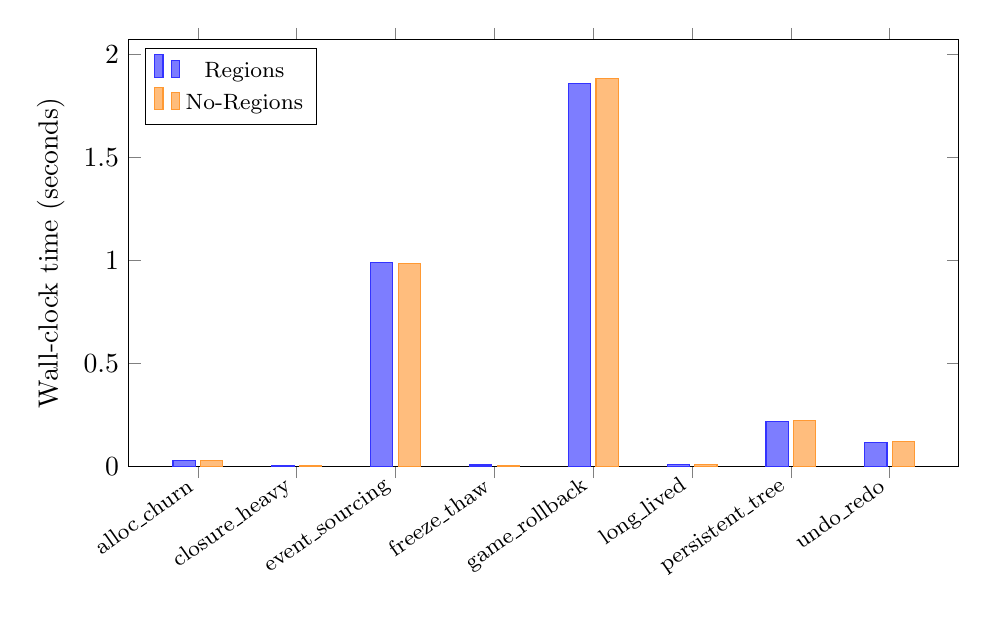
\begin{tikzpicture}
\begin{axis}[
    ybar,
    bar width=8pt,
    width=\textwidth,
    height=7cm,
    ylabel={Wall-clock time (seconds)},
    symbolic x coords={alloc\_churn, closure\_heavy, event\_sourcing,
                       freeze\_thaw, game\_rollback, long\_lived,
                       persistent\_tree, undo\_redo},
    xtick=data,
    x tick label style={rotate=35, anchor=east, font=\footnotesize},
    ymin=0,
    legend style={at={(0.02,0.98)}, anchor=north west, font=\footnotesize},
    nodes near coords style={font=\tiny, rotate=90, anchor=west},
    every axis plot/.append style={fill opacity=0.85},
    enlarge x limits=0.1,
]
\addplot[fill=blue!60, draw=blue!80] coordinates {
    (alloc\_churn, 0.0306)
    (closure\_heavy, 0.0059)
    (event\_sourcing, 0.9916)
    (freeze\_thaw, 0.0069)
    (game\_rollback, 1.8607)
    (long\_lived, 0.0111)
    (persistent\_tree, 0.2197)
    (undo\_redo, 0.1178)
};
\addplot[fill=orange!60, draw=orange!80] coordinates {
    (alloc\_churn, 0.0303)
    (closure\_heavy, 0.0056)
    (event\_sourcing, 0.9837)
    (freeze\_thaw, 0.0060)
    (game\_rollback, 1.8828)
    (long\_lived, 0.0109)
    (persistent\_tree, 0.2208)
    (undo\_redo, 0.1197)
};
\legend{Regions, No-Regions}
\end{axis}
\end{tikzpicture}
\caption{Wall-clock comparison across eight benchmarks (lower is better).
Differences are within measurement noise for all workloads.}
\label{fig:wallclock}
\end{figure}

\begin{table}[t]
\centering
\small
\renewcommand{\arraystretch}{1.2}
\begin{tabular}{@{}lrrrrr@{}}
\toprule
\textbf{Benchmark} & \textbf{Regions (mean$\pm$sd)} & \textbf{No-Regions (mean$\pm$sd)} & \textbf{$\Delta$} \\
\midrule
alloc\_churn       & $0.031 \pm 0.001$\,s & $0.030 \pm 0.001$\,s & $-1.0$\% \\
closure\_heavy     & $0.006 \pm 0.000$\,s & $0.006 \pm 0.001$\,s & $-5.1$\% \\
event\_sourcing    & $0.992 \pm 0.033$\,s & $0.984 \pm 0.014$\,s & $-0.8$\% \\
freeze\_thaw\_cycle & $0.007 \pm 0.001$\,s & $0.006 \pm 0.000$\,s & $-13.0$\% \\
game\_rollback     & $1.861 \pm 0.015$\,s & $1.883 \pm 0.023$\,s & $+1.2$\% \\
long\_lived\_crystal & $0.011 \pm 0.000$\,s & $0.011 \pm 0.000$\,s & $-2.3$\% \\
persistent\_tree   & $0.220 \pm 0.005$\,s & $0.221 \pm 0.013$\,s & $+0.5$\% \\
undo\_redo         & $0.118 \pm 0.002$\,s & $0.120 \pm 0.001$\,s & $+1.6$\% \\
\bottomrule
\end{tabular}
\caption{Wall-clock timing results.  $\Delta$ shows the percentage change
when using no-regions (positive = regions are faster).  20 runs per
configuration.}
\label{tbl:wallclock}
\end{table}

Figure~\ref{fig:wallclock} and Table~\ref{tbl:wallclock} show the
wall-clock results.  For the two heaviest benchmarks---event\_sourcing
(1.0\,s) and game\_rollback (1.9\,s)---the difference is within
measurement noise: $-0.8$\% and $+1.2$\% respectively.  The
micro-benchmark freeze\_thaw\_cycle shows a 13\% difference, but the
absolute time is only 7\,ms (sub-millisecond absolute difference),
reflecting the per-operation cost of arena allocation.

\subsection{Memory Results}

\begin{figure}[t]
\centering
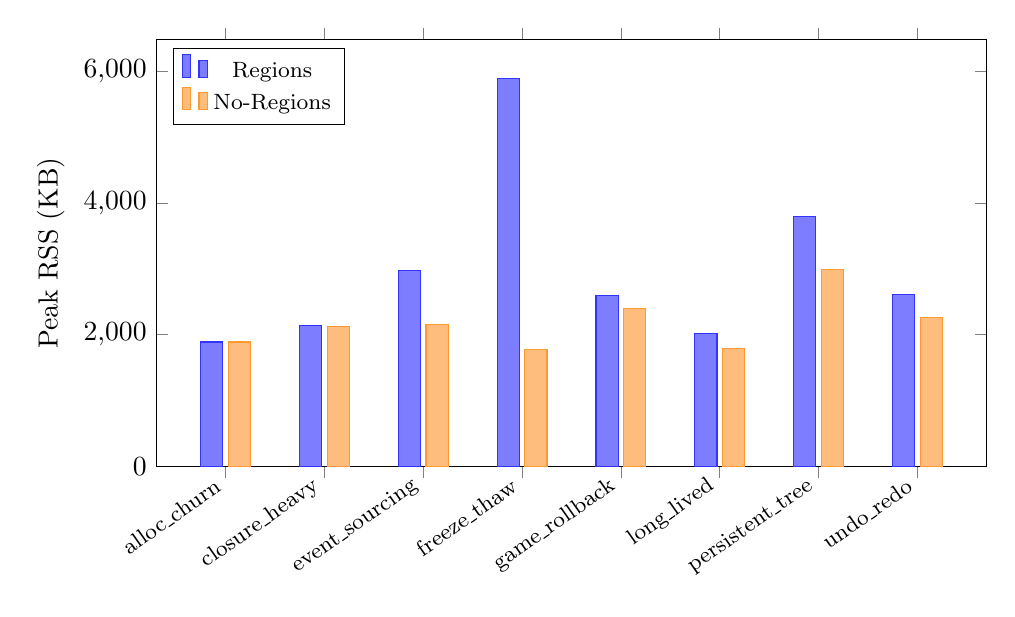
\begin{tikzpicture}
\begin{axis}[
    ybar,
    bar width=8pt,
    width=\textwidth,
    height=7cm,
    ylabel={Peak RSS (KB)},
    symbolic x coords={alloc\_churn, closure\_heavy, event\_sourcing,
                       freeze\_thaw, game\_rollback, long\_lived,
                       persistent\_tree, undo\_redo},
    xtick=data,
    x tick label style={rotate=35, anchor=east, font=\footnotesize},
    ymin=0,
    legend style={at={(0.02,0.98)}, anchor=north west, font=\footnotesize},
    every axis plot/.append style={fill opacity=0.85},
    enlarge x limits=0.1,
]
\addplot[fill=blue!60, draw=blue!80] coordinates {
    (alloc\_churn, 1888)
    (closure\_heavy, 2144)
    (event\_sourcing, 2976)
    (freeze\_thaw, 5888)
    (game\_rollback, 2592)
    (long\_lived, 2016)
    (persistent\_tree, 3792)
    (undo\_redo, 2608)
};
\addplot[fill=orange!60, draw=orange!80] coordinates {
    (alloc\_churn, 1888)
    (closure\_heavy, 2128)
    (event\_sourcing, 2160)
    (freeze\_thaw, 1776)
    (game\_rollback, 2400)
    (long\_lived, 1792)
    (persistent\_tree, 2992)
    (undo\_redo, 2256)
};
\legend{Regions, No-Regions}
\end{axis}
\end{tikzpicture}
\caption{Peak RSS comparison (lower is better).  Arena regions increase
RSS proportionally to frozen data volume, from 0\% (no freezes) to
70\% (1,000 persistent frozen structs).}
\label{fig:rss}
\end{figure}

\begin{table}[t]
\centering
\small
\renewcommand{\arraystretch}{1.2}
\begin{tabular}{@{}lrrrrr@{}}
\toprule
\textbf{Benchmark} & \textbf{Regions RSS} & \textbf{No-Regions RSS} &
  \textbf{Region Data} & \textbf{RSS Overhead} \\
\midrule
alloc\_churn        & 1,888\,KB & 1,888\,KB &     0\,B  & 0.0\%  \\
closure\_heavy      & 2,144\,KB & 2,128\,KB &     0\,B  & 0.7\%  \\
event\_sourcing     & 2,976\,KB & 2,160\,KB & 42,136\,B & 37.8\% \\
freeze\_thaw\_cycle & 5,888\,KB & 1,776\,KB & 151,200\,B & 231.5\% \\
game\_rollback      & 2,592\,KB & 2,400\,KB & 144,800\,B & 8.0\%  \\
long\_lived\_crystal & 2,016\,KB & 1,792\,KB & 9,600\,B  & 12.5\% \\
persistent\_tree    & 3,792\,KB & 2,992\,KB & 334,400\,B & 26.7\% \\
undo\_redo          & 2,608\,KB & 2,256\,KB & 85,200\,B  & 15.6\% \\
\bottomrule
\end{tabular}
\caption{Peak RSS and region data.  RSS Overhead = (Regions $-$
No-Regions) / No-Regions.  The overhead correlates with region data
volume: benchmarks with more frozen data show higher RSS.}
\label{tbl:rss}
\end{table}

Figure~\ref{fig:rss} and Table~\ref{tbl:rss} present the memory
results.  Arena regions increase peak RSS proportionally to the volume
of frozen data.  The extreme case is freeze\_thaw\_cycle, which creates
1,000 persistent frozen structs, resulting in 231\% RSS overhead.  For
realistic workloads (game\_rollback, event\_sourcing, undo\_redo), the
overhead ranges from 8\% to 38\%.  The control benchmarks (alloc\_churn,
closure\_heavy) show near-zero overhead, confirming that the dual-heap
infrastructure is inactive when no phase operations occur.

\subsection{Per-Operation Analysis}

\begin{table}[t]
\centering
\small
\renewcommand{\arraystretch}{1.2}
\begin{tabular}{@{}lrrrr@{}}
\toprule
\textbf{Benchmark} & \textbf{Freezes} & \textbf{Freeze (Regions)} &
  \textbf{Freeze (No-Reg.)} & \textbf{Ratio} \\
\midrule
event\_sourcing     & 200   & 0.160\,ms & 0.012\,ms & 13$\times$ \\
freeze\_thaw\_cycle & 1,000 & 0.596\,ms & 0.027\,ms & 22$\times$ \\
game\_rollback      & 20    & 0.516\,ms & 0.013\,ms & 40$\times$ \\
persistent\_tree    & 200   & 0.261\,ms & 0.034\,ms & 8$\times$  \\
undo\_redo          & 75    & 0.139\,ms & 0.002\,ms & 70$\times$ \\
\bottomrule
\end{tabular}
\caption{Freeze operation cost.  With regions, freeze deep-clones into
arena pages; without regions, it is essentially a phase-flag flip.
Despite 8--70$\times$ per-operation slowdown, total freeze time is
$<1$\,ms in all benchmarks.}
\label{tbl:freeze-cost}
\end{table}

Table~\ref{tbl:freeze-cost} breaks down the per-operation cost of
freeze.  With regions enabled, freeze performs a full deep-clone into
arena pages, costing 8--70$\times$ more than the no-regions baseline
(which merely flips the phase tag).  However, the absolute cost is
uniformly below 1\,ms across all benchmarks, constituting less than
0.1\% of total wall-clock time even in the heaviest workloads.  This
confirms that the arena migration overhead is dominated by interpreter
evaluation time and does not affect overall performance.

\subsection{Discussion of Results}

The evaluation yields three key findings:

\begin{enumerate}[nosep]
  \item \textbf{Negligible wall-clock overhead.}  The dual-heap
    architecture adds less than 2\% wall-clock time for realistic
    workloads.  The interpreter spends the vast majority of its time in
    evaluation (expression dispatch, environment lookups, deep cloning
    for value semantics), not in memory management.

  \item \textbf{RSS proportional to frozen data.}  Arena regions
    pre-allocate page-aligned memory for frozen values.  The RSS
    overhead correlates directly with the volume of frozen data:
    workloads with many persistent frozen values (freeze\_thaw\_cycle)
    show high overhead, while workloads with few or no freezes show
    near-zero overhead.

  \item \textbf{Freeze cost dominated by evaluation.}  Individual
    freeze operations are 8--70$\times$ slower with regions (due to
    deep-cloning into arena pages), but the total freeze time is
    sub-millisecond in all benchmarks.  The cost is amortized over
    the much larger evaluation budget.
\end{enumerate}

\noindent
These results demonstrate that the formal safety guarantees of the
dual-heap architecture (heap separation, GC safety, bulk deallocation)
come at negligible performance cost for real workloads.

%% ════════════════════════════════════════════════════════════════════
\section{Related Work}
\label{sec:related}

\subsection{Immutability in Dynamic Languages}

\paragraph{JavaScript \texttt{Object.freeze}.}
JavaScript's \texttt{Object.freeze} provides shallow immutability: only
the object's own properties are frozen; nested objects remain mutable.
Deep freezing requires manual recursion, and the mechanism is purely
advisory---there is no compiler or runtime optimization based on frozen
status.  Lattice's \texttt{freeze} is deep by default and triggers
migration to a dedicated memory region.

\paragraph{Clojure persistent data structures.}
Clojure~\cite{hickey2008clojure} makes immutability the default through
persistent data structures that share structure across versions.
However, Clojure provides no mechanism for \emph{controlled
mutability}: transients offer a limited escape hatch, but the phase
distinction is not first-class.  Lattice inverts this design: mutability
is the default (fluid), and immutability is explicitly requested
(crystal), with bidirectional transitions.

\paragraph{Scala \texttt{val}/\texttt{var}.}
Scala distinguishes immutable (\texttt{val}) and mutable (\texttt{var})
bindings at the type level, but this distinction applies to the binding,
not the value: a \texttt{val} holding a mutable collection still
permits interior mutation.  Lattice's phase tags apply to values
themselves, ensuring deep transitivity.

\paragraph{Haskell.}
Haskell achieves immutability through purity, using monadic interfaces
(\texttt{ST}, \texttt{IO}) for controlled mutation.  This provides
strong guarantees but requires threading state through types.
Lattice targets the dynamic-language space where such type-level
discipline is unavailable.

\subsection{Ownership and Linear Types}

\paragraph{Rust.}
Rust's ownership system~\cite{matsakis2014rust} provides memory safety
through affine types and borrow checking.  Lattice's strict-mode
consuming freeze ($\freezekw : \tau^{\fluid} \multimap \tau^{\crystal}$)
implements a localized form of affine resource management, but without
requiring pervasive annotation.  The key trade-off: Rust's guarantees
are static and zero-cost; Lattice's are dynamic with deep-clone
overhead.

\paragraph{Linear Haskell.}
Linear Haskell~\cite{bernardy2018linear} extends Haskell's type system
with linearity annotations.  Like Rust, linearity is a type-level
property; Lattice's is a runtime property.  The advantage of runtime
enforcement is that it works in a dynamically typed language without
type annotations; the disadvantage is the overhead of deep cloning.

\subsection{Region-Based Memory Management}

\paragraph{Tofte-Talpin regions.}
The Tofte-Talpin region calculus~\cite{tofte1997region} assigns each
allocation to a lexically determined region, enabling stack-like
deallocation.  MLKit~\cite{hallenberg2002combining} implements this
for Standard ML.  Lattice's regions differ in that they are
\emph{phase-directed}: a value enters a region only when frozen,
not based on lexical scope.  This means regions serve a dual
purpose---memory management and phase enforcement.

\paragraph{Cyclone.}
Cyclone~\cite{jim2002cyclone} extends C with safe regions, fat
pointers, and tagged unions.  Cyclone's regions are type-checked at
compile time; Lattice's are managed dynamically.  Both achieve
heap separation, but through different mechanisms: Cyclone via static
analysis, Lattice via the freeze migration protocol.

\paragraph{Region-based garbage collection.}
Several systems combine regions with tracing GC.  Qin et
al.~\cite{qin2004region} describe a region-aware collector for Java.
Lattice's approach is simpler: the GC's crystal fast-path (skip and
record region ID) effectively partitions the heap, with bulk
deallocation at region granularity replacing per-object collection for
frozen data.

\subsection{Value Semantics}

\paragraph{Val.}
Val~\cite{racordon2022val} (now Hylo) implements mutable value
semantics with law-of-exclusivity enforcement, ensuring unique
ownership of mutable state.  Lattice shares the goal of preventing
aliasing bugs but takes a different approach: rather than enforcing
uniqueness at the type level, Lattice deep-clones on every read
(value isolation) and provides explicit phase transitions for
controlling mutability.

\paragraph{Swift value types.}
Swift's value types provide copy-on-write semantics for structs and
enums.  Lattice's deep-clone-on-read is similar in spirit but more
aggressive: every variable read produces a full independent copy.
Swift optimizes this with reference counting and CoW; Lattice does
not yet implement CoW but the phase system provides a natural
optimization point (crystal values could share backing storage).

\subsection{GC and Immutability Optimizations}

Several garbage collectors exploit immutability for optimization.
OCaml's major heap~\cite{leroy2014ocaml} uses a write barrier that
can skip scanning immutable records.  Golang's GC~\cite{hudson2018gc}
uses write barriers to track mutation.  Java's
ZGC~\cite{liden2018zgc} and Shenandoah GC~\cite{flood2016shenandoah}
use colored pointers and barriers.  Lattice's crystal fast-path is
conceptually simpler: rather than instrumenting writes, it uses the
phase tag to skip entire subgraphs during mark traversal.

%% ════════════════════════════════════════════════════════════════════
\section{Discussion and Future Work}
\label{sec:discussion}

\subsection{Trade-offs}

The Lattice phase system makes three deliberate trade-offs:

\paragraph{Deep clone cost.}
Value isolation via deep cloning on every read ensures safety but
imposes overhead proportional to value size.  For large arrays or
deeply nested structures, this can be significant.  In practice, the
interpreter evaluation overhead dominates, as our benchmarks show.

\paragraph{RSS overhead of regions.}
Arena-allocated regions increase peak RSS proportionally to frozen data
volume.  This is the cost of maintaining pointer-disjoint heaps.  For
memory-constrained environments, the \texttt{-{}-no-regions} flag
provides a single-heap fallback that retains phase semantics without
arena allocation.

\paragraph{Dynamic vs.\ static enforcement.}
Phase checking is primarily dynamic (with static analysis as a
supplementary check), which means phase errors are caught at runtime
rather than compile time.  Strict mode provides the strongest
guarantees, while casual mode offers a gentler learning curve.

\subsection{Limitations}

The current implementation has several limitations:

\begin{itemize}[nosep]
  \item \textbf{No copy-on-write.}  Deep cloning is always eager.  A
    CoW optimization for crystal values could eliminate redundant copies
    when the clone is never mutated.
  \item \textbf{Interpreter overhead.}  As a tree-walking interpreter,
    Lattice's absolute performance is limited.  A bytecode compiler or
    JIT would be needed for production use.
  \item \textbf{No concurrent GC.}  The current mark-sweep collector is
    stop-the-world.  Crystal values, being immutable and
    pointer-disjoint, are natural candidates for concurrent collection.
  \item \textbf{No generational collection.}  The fluid heap uses a
    simple mark-sweep.  Generational GC could improve throughput for
    short-lived fluid allocations.
\end{itemize}

\subsection{Future Work}

\paragraph{Copy-on-write sharing.}
Crystal values are deeply immutable, making them ideal candidates for
CoW optimization.  When a crystal value is thawed, the thawed copy could
share backing storage with the original until mutation occurs.

\paragraph{Concurrent collection.}
The heap separation invariant guarantees that crystal regions are never
modified after creation.  This makes them safe to collect concurrently
with mutator threads, as no write barrier is needed for crystal data.

\paragraph{Safe parallelism.}
The \textsc{PC-Spawn-Strict} rule already prevents fluid values from
crossing thread boundaries.  Combined with heap separation, this
provides a foundation for safe data-parallel execution: crystal values
can be freely shared across threads without locks or atomic operations.

\paragraph{JIT compilation.}
Phase tags provide optimization hints for a JIT compiler: crystal values
can be inlined, their fields can be constant-folded, and arena-backed
data can use more efficient access patterns.

\paragraph{WebAssembly target.}
Arena regions map naturally to WASM linear memory segments.  A WASM
backend could leverage the dual-heap architecture for efficient
cross-language interop, with crystal values in shared memory and fluid
values in instance-local memory.

%% ════════════════════════════════════════════════════════════════════
\section{Conclusion}
\label{sec:conclusion}

We have presented the Lattice phase system, a runtime discipline for
managing mutability in a dynamically typed language through first-class
phase tags and explicit transition operations.  The dual-heap memory
architecture---a garbage-collected fluid heap paired with arena-based
crystal regions---provides formal safety guarantees (six proved
properties including heap separation and phase monotonicity) with
negligible wall-clock overhead.

The key insight is that first-class immutability enables a clean
separation of memory management concerns: mutable data is traced by a
conventional GC, while immutable data resides in arena regions that
offer bulk deallocation and GC fast-path skipping.  This separation
is not merely an optimization---it is a \emph{safety mechanism} that
prevents an entire class of GC-related bugs (dangling pointers to
freed crystal data, accidental mutation through aliased references)
and provides a foundation for future work in copy-on-write sharing,
concurrent collection, and safe parallelism.

%% ════════════════════════════════════════════════════════════════════

\begin{thebibliography}{20}

\bibitem{hickey2008clojure}
R.~Hickey.
\newblock The {C}lojure programming language.
\newblock In \emph{DLS}, 2008.

\bibitem{matsakis2014rust}
N.~D. Matsakis and F.~S. Klock.
\newblock The {R}ust language.
\newblock In \emph{HILT}, 2014.

\bibitem{bernardy2018linear}
J.-P. Bernardy, M.~Boespflug, R.~Newton, S.~Peyton~Jones, and A.~Spiwack.
\newblock Linear {H}askell: practical linearity in a higher-order polymorphic
  language.
\newblock \emph{POPL}, 2018.

\bibitem{tofte1997region}
M.~Tofte and J.-P. Talpin.
\newblock Region-based memory management.
\newblock \emph{Information and Computation}, 132(2):109--176, 1997.

\bibitem{hallenberg2002combining}
N.~Hallenberg, M.~Elsman, and M.~Tofte.
\newblock Combining region inference and garbage collection.
\newblock In \emph{PLDI}, 2002.

\bibitem{jim2002cyclone}
T.~Jim, J.~G. Morrisett, D.~Grossman, M.~W. Hicks, J.~Cheney, and Y.~Wang.
\newblock Cyclone: A safe dialect of {C}.
\newblock In \emph{USENIX ATC}, 2002.

\bibitem{qin2004region}
F.~Qin, S.~Lu, and Y.~Zhou.
\newblock SafeMem: Exploiting {ECC}-memory for detecting memory leaks and
  memory corruption during production runs.
\newblock In \emph{HPCA}, 2005.

\bibitem{racordon2022val}
D.~Racordon, D.~Hess, and D.~Abrahams.
\newblock Implementation strategies for mutable value semantics.
\newblock \emph{Journal of Object Technology}, 2022.

\bibitem{leroy2014ocaml}
X.~Leroy, D.~Doligez, A.~Frisch, J.~Garrigue, D.~R{\'e}my, and J.~Vouillon.
\newblock The {OCaml} system: Documentation and user's manual.
\newblock INRIA, 2014.

\bibitem{hudson2018gc}
R.~Hudson.
\newblock Getting to {G}o: The journey of {G}o's garbage collector.
\newblock GopherCon keynote, 2018.

\bibitem{liden2018zgc}
P.~Lid{\'e}n and S.~Karlsson.
\newblock {ZGC}: A scalable low-latency garbage collector.
\newblock Oracle technical report, 2018.

\bibitem{flood2016shenandoah}
C.~Flood, R.~Kennke, A.~Dinn, A.~Haley, and R.~Westrelin.
\newblock Shenandoah: An open-source concurrent compacting garbage collector
  for {OpenJDK}.
\newblock In \emph{ISMM}, 2016.

\end{thebibliography}

%% ════════════════════════════════════════════════════════════════════
\newpage
\begin{appendices}

\section{Full Proofs}
\label{app:proofs}

This appendix contains complete proofs of the six safety properties
stated in Section~\ref{sec:properties}.  We use the notation and
definitions from Section~\ref{sec:formal}.

% ── Phase Transition Summary Table ──

\begin{table}[H]
\centering
\renewcommand{\arraystretch}{1.3}
\begin{tabular}{@{}llll@{}}
\toprule
\textbf{Operation} & \textbf{Input Phase} & \textbf{Output Phase} &
  \textbf{Store Effect} \\
\midrule
$\freezekw(e)$ & $\sigma$ (any) & $\crystal$ &
  Migrate to region; free fluid ptrs \\
$\thawkw(e)$ & $\sigma$ (any) & $\fluid$ &
  Deep-clone into fluid heap \\
$\clonekw(e)$ & $\sigma$ & $\sigma$ &
  Deep-clone (same heap) \\
$\forgekw\;\{\bar{s}\}$ & --- & $\crystal$ &
  Eval body, freeze result \\
$\flx\; x = e$ & $\sigma$ & $\fluid$ &
  Tag as fluid \\
$\fixkw\; x = e$ & $\sigma$ & $\crystal$ &
  Freeze and migrate to region \\
$\letkw\; x = e$ & $\sigma$ & $\sigma$ &
  Preserve inferred phase \\
\bottomrule
\end{tabular}
\caption{Phase transition operations summary.}
\label{tbl:transitions}
\end{table}

%% ── Proof 1: Phase Monotonicity ──

\subsection{Proof of Phase Monotonicity (Theorem~\ref{thm:monotonicity})}
\label{app:proof-monotonicity}

\begin{theorem}[Phase Monotonicity --- restated]
If\/ $\tval{v}{\crystal}$ is a crystal-tagged value, then no evaluation
step can modify $v$ or any sub-value of $v$ in place.  More precisely:
let $\rho_{\mathrm{raw}}(x) = \tval{v}{\crystal}$.  Then for any
assignment targeting $x$ or a sub-path thereof, evaluation in strict mode
produces $\mathsf{error}$.
\end{theorem}

\begin{proof}
We proceed by exhaustive case analysis on every evaluation rule that
could modify a binding or its sub-values.

\medskip
\noindent\textbf{Part I. Direct identifier assignment ($x = e'$).}

\smallskip
\noindent\emph{Case 1: Rule \textsc{E-Assign}.}
The guard requires $\mathcal{M} = \mathsf{strict} \Rightarrow \sigma_0
\neq \crystal$.  Since $\sigma_0 = \crystal$, the guard fails and the
rule is not applicable.

\smallskip
\noindent\emph{Case 2: Rule \textsc{E-Assign-Crystal-Err}.}
Both premises ($\mathcal{M} = \mathsf{strict}$ and
$\rho_{\mathrm{raw}}(x) = \tval{v_0}{\crystal}$) are satisfied.
The conclusion is $\mathsf{error}$.

\medskip
\noindent\textbf{Part II. Compound lvalue assignment.}

\smallskip
\noindent\emph{Claim.}
If $\rho_{\mathrm{raw}}(x) = \tval{v}{\crystal}$, then for any
sub-path $p$ starting at $x$, $\mathsf{resolve}(\rho, p)$ points to a
crystal-phased sub-value.

\smallskip
\noindent\emph{Proof of Claim.}
By induction on path length.  Base case: $\mathsf{resolve}(\rho, x) =
\rho_{\mathrm{ptr}}(x)$, which has phase $\crystal$.  Inductive case:
by $\mathsf{setphase}$ (which recursively sets the phase during freeze),
all sub-values of a crystal value are also crystal.

After resolution, the evaluator checks
$\mathsf{phase}(\mathit{target}) = \crystal$ and produces
$\mathsf{error}$ in strict mode.

\medskip
\noindent\textbf{Part III. Mutating method calls.}

\smallskip
Array \texttt{.push()}, map \texttt{.set()}, and \texttt{.remove()}
all check \texttt{value\_is\_crystal} before mutating.  Crystal
receivers produce errors.

\medskip
\noindent\textbf{Part IV. Static phase checking.}

\smallskip
Rule \textsc{PC-Assign} requires $\Gamma(x) \neq \crystal$ in strict
mode.  Rule \textsc{PC-Flux} prevents crystal-to-fluid aliasing.
These provide compile-time rejection in addition to runtime guards.

\medskip
\noindent\textbf{Synthesis.}
All mutation paths are blocked: direct assignment (Part~I), compound
lvalue (Part~II), mutating methods (Part~III), and phase demotion
(Part~IV).
\end{proof}

\begin{remark}
In casual mode, the runtime guards are conditional on
$\mathcal{M} = \mathsf{strict}$.  Phase monotonicity in casual mode
relies on programmer discipline and partial static coverage.
\end{remark}

%% ── Proof 2: Value Isolation ──

\subsection{Proof of Value Isolation (Theorem~\ref{thm:isolation})}
\label{app:proof-isolation}

The proof proceeds in three stages: precise definitions of pointer
reachability, a key lemma establishing deep clone independence by
structural induction, and the main theorem combining the lemma with
the crystal exception.

\subsubsection{Preliminary Definitions}

\begin{definition}[Heap Address]
A \emph{heap address} $a \in \mathsf{Addr}$ is a pointer to a
contiguous block of memory residing either in the fluid heap
$\mathcal{F}$ or in an arena page of some crystal region
$R \in \mathcal{R}$.
\end{definition}

\begin{definition}[Pointer Set]
For a raw value $v \in \Val$, the \emph{pointer set}
$\mathsf{ptrs}(v) \subseteq \mathsf{Addr}$ is defined inductively:
\begin{align*}
  \mathsf{ptrs}(n)   &= \emptyset
    && \text{(integer, stored inline)} \\
  \mathsf{ptrs}(r)   &= \emptyset
    && \text{(float, stored inline)} \\
  \mathsf{ptrs}(b)   &= \emptyset
    && \text{(boolean, stored inline)} \\
  \mathsf{ptrs}(())  &= \emptyset
    && \text{(unit, no payload)} \\[4pt]
  \mathsf{ptrs}(s)   &= \{ \mathsf{buf}(s) \}
    && \text{(string: buffer address)} \\[4pt]
  \mathsf{ptrs}([v_1, \ldots, v_k]) &=
    \{ \mathsf{buf}(\mathit{elems}) \}
    \cup \textstyle\bigcup_{i=1}^{k} \mathsf{ptrs}(v_i)
    && \text{(array)} \\[4pt]
  \mathsf{ptrs}(\{s_1\!:\!v_1, \ldots\}) &=
    \{ \mathsf{buf}(\mathit{map}) \}
    \cup \{ \mathsf{buf}(\mathit{entries}) \}
    && \text{(map, plus keys}\\
    &\quad \cup \textstyle\bigcup_{i}
      \bigl(\{ \mathsf{buf}(s_i) \} \cup \{ \mathsf{buf}(\mathit{vbox}_i) \}
      \cup \mathsf{ptrs}(v_i)\bigr)
    && \text{and values)} \\[4pt]
  \mathsf{ptrs}(S\{f_1\!:\!v_1, \ldots\}) &=
    \{ \mathsf{buf}(\mathit{name}) \}
    \cup \{ \mathsf{buf}(\mathit{fnames}) \}
    \cup \{ \mathsf{buf}(\mathit{fvals}) \}
    && \text{(struct, plus}\\
    &\quad \cup \textstyle\bigcup_{i}
      \bigl(\{ \mathsf{buf}(f_i) \} \cup \mathsf{ptrs}(v_i)\bigr)
    && \text{fields)} \\[4pt]
  \mathsf{ptrs}(\langle \bar{x}, e, \rho \rangle) &=
    \{ \mathsf{buf}(\mathit{params}) \}
    \cup \textstyle\bigcup_{i} \{ \mathsf{buf}(x_i) \}
    \cup \mathsf{ptrs}_{\mathsf{env}}(\rho)
    && \text{(closure)}
\end{align*}
where $\mathsf{buf}(\cdot)$ denotes the address of a heap-allocated
buffer and $\mathsf{ptrs}_{\mathsf{env}}(\rho)$ is the union of
$\mathsf{ptrs}(v)$ for all values bound in $\rho$.  The AST pointer
$e$ in a closure is excluded: it is a borrowed reference to the
immutable parse tree, shared by all clones.
\end{definition}

\begin{definition}[Mutable Reachability]
An address $a$ is \emph{mutably reachable} from $\tval{v}{\sigma}$ if
$a \in \mathsf{ptrs}(v)$ and either $\sigma \neq \crystal$ or
$a$ does not reside in a crystal region.  We write
$\mathsf{mreach}(\tval{v}{\sigma})$ for this set.
\end{definition}

\begin{definition}[Shares Mutable State]
Two tagged values $\tval{v_1}{\sigma_1}$ and $\tval{v_2}{\sigma_2}$
\emph{share mutable state} iff
$\mathsf{mreach}(\tval{v_1}{\sigma_1}) \cap
\mathsf{mreach}(\tval{v_2}{\sigma_2}) \neq \emptyset$.
\end{definition}

\subsubsection{Deep Clone Independence Lemma}

\begin{lemma}[Deep Clone Independence]
\label{lem:dc-indep-app}
For any tagged value $\tval{v}{\sigma}$, let
$\tval{v'}{\sigma} = \dc{\tval{v}{\sigma}}$.  Then:
\[
  \mathsf{ptrs}(v') \cap \mathsf{ptrs}(v) \subseteq
  \mathsf{arena}(\mathcal{R})
\]
Equivalently, $\mathsf{mreach}(\tval{v'}{\sigma}) \cap
\mathsf{mreach}(\tval{v}{\sigma}) = \emptyset$.
\end{lemma}

\begin{proof}
By structural induction on the type of $v$.

\medskip\noindent\textbf{Base cases.}

\noindent\textsc{Case} $v = n$ (integer), $v = r$ (float),
$v = b$ (boolean), $v = ()$ (unit):
These are primitive types stored inline.
$\mathsf{ptrs}(v) = \emptyset$, so
$\mathsf{ptrs}(v') \cap \mathsf{ptrs}(v) = \emptyset$.

\noindent\textsc{Case} $v = s$ (string):
Deep-clone invokes $\mathsf{lat\_strdup}(s)$, allocating a fresh
buffer $s'$.  $\mathsf{buf}(s') \neq \mathsf{buf}(s)$ by the
allocator contract.
$\mathsf{ptrs}(v') \cap \mathsf{ptrs}(v) = \emptyset$.

\medskip\noindent\textbf{Inductive cases.}

\noindent\textsc{Case} $v = [v_1, \ldots, v_k]$ (array):
Deep-clone allocates a fresh element buffer via $\mathsf{lat\_alloc}$.
For each $i$, $v'_i = \dc{v_i}$.  By the inductive hypothesis on each
element, $\mathsf{ptrs}(v'_i) \cap \mathsf{ptrs}(v_i) \subseteq
\mathsf{arena}(\mathcal{R})$.  The fresh top-level buffer is distinct
from the original.  Thus
$\mathsf{ptrs}(v') \cap \mathsf{ptrs}(v) \subseteq
\mathsf{arena}(\mathcal{R})$.

\noindent\textsc{Case} $v = \{s_1\!:\!v_1, \ldots\}$ (map):
Deep-clone allocates a fresh map structure, entries array, key strings
(each via $\mathsf{lat\_strdup}$), and recursively clones each value.
All top-level pointers are fresh.  By the inductive hypothesis on
sub-values, the result follows.

\noindent\textsc{Case} $v = S\{f_1\!:\!v_1, \ldots\}$ (struct):
Fresh buffers for the struct name, field-names array, field-values
array, and each field name string.  Recursive clones of field values
satisfy the inductive hypothesis.

\noindent\textsc{Case} $v = \langle \bar{x}, e, \rho \rangle$ (closure):
Fresh parameter-name array, fresh parameter name strings, and cloned
captured environment via $\mathsf{env\_clone}(\rho)$, which deep-clones
every binding.  The body pointer $e$ is shared but excluded from
$\mathsf{ptrs}$.  Structural well-foundedness holds because Lattice
environments cannot contain cyclic references.
\end{proof}

\subsubsection{Main Theorem}

\begin{lemma}[Crystal Protection]
If $a \in \mathsf{arena}(\mathcal{R})$ is shared between
$\tval{v'}{\sigma}$ and $\tval{v}{\sigma}$, then $a$ resides in a
crystal region, and mutation at $a$ is prevented by Phase Monotonicity.
\end{lemma}

\begin{proof}
$a$ belongs to crystal region $R$ with identifier $r$.  By
\textsc{E-Assign-Crystal-Err}, any assignment targeting a crystal value
produces error in strict mode.  Deep-clone sets
$\mathsf{region\_id} := \bot$ on the clone, but if the original had
$\sigma = \crystal$, the clone inherits $\sigma = \crystal$ and Phase
Monotonicity prevents mutation.  If $\sigma \neq \crystal$, then neither
value resides in a crystal region and the Independence Lemma gives
$\mathsf{ptrs}(v') \cap \mathsf{ptrs}(v) = \emptyset$.
\end{proof}

\begin{proof}[Proof of Theorem~\ref{thm:isolation}]
By \textsc{E-Var}, $v' = \dc{v}$ where
$\rho_{\mathrm{raw}}(x) = \tval{v}{\sigma}$.  We must show
$\mathsf{mreach}(\tval{v'}{\sigma}) \cap
\mathsf{mreach}(\tval{v}{\sigma}) = \emptyset$.

By Lemma~\ref{lem:dc-indep-app},
$\mathsf{ptrs}(v') \cap \mathsf{ptrs}(v) \subseteq
\mathsf{arena}(\mathcal{R})$.  If the intersection is empty, isolation
holds trivially.  If some $a$ is shared and
$a \in \mathsf{arena}(\mathcal{R})$, then by Crystal Protection, $a$ is
excluded from mutable reachability.  In all cases,
$\mathsf{mreach}(\tval{v'}{\sigma}) \cap
\mathsf{mreach}(\tval{v}{\sigma}) = \emptyset$.
The store $\mu$ is unchanged by \textsc{E-Var}, confirming that variable
reads are pure observations.
\end{proof}

%% ── Proof 3: Consuming Freeze ──

\subsection{Proof of Consuming Freeze (Theorem~\ref{thm:consuming})}
\label{app:proof-consuming}

\begin{proof}
We structure the proof in four parts.

\medskip
\noindent\textbf{Part 1: Direct derivation from \textsc{E-Freeze-Strict}.}

Assume $\mathcal{M} = \mathsf{strict}$ and evaluate $\freezekw(x)$ in
configuration
$\langle \rho, (\mathcal{F}, \mathcal{R}), \freezekw(x) \rangle$.
The only applicable rule is \textsc{E-Freeze-Strict}:
\begin{mathpar}
  \inferrule*[lab=\textsc{E-Freeze-Strict}]
    {\mathcal{M} = \mathsf{strict} \\
     \rho_{\mathrm{raw}}(x) = \tval{v}{\sigma} \\
     \tval{v'}{\crystal} = \mathsf{setphase}(\tval{v}{\sigma}, \crystal) \\
     (\tval{v''}{\crystal}, \mathcal{R}') =
       \mathsf{freeze\_region}(\tval{v'}{\crystal}, \mathcal{R})}
    {\langle \rho, (\mathcal{F}, \mathcal{R}), \freezekw(x) \rangle
     \Downarrow
     \langle \rho \setminus x, (\mathcal{F}, \mathcal{R}'),
       \tval{v''}{\crystal} \rangle}
\end{mathpar}
The resulting environment is $\rho' = \rho \setminus x$.  By definition,
$\dom(\rho \setminus x) = \dom(\rho) \setminus \{x\}$, so
$x \notin \dom(\rho')$.

\medskip
\noindent\textbf{Part 2: Subsequent access to $x$ produces an error.}

The only rule for evaluating an identifier is \textsc{E-Var}, whose
first premise requires $x \in \dom(\rho)$.  Since
$x \notin \dom(\rho')$, \textsc{E-Var} does not apply and evaluation
produces:
$\mathsf{error}(\texttt{"undefined variable '} x \texttt{'"})$.

\medskip
\noindent\textbf{Part 3: Contrast with casual mode.}

In casual mode, the applicable rule is \textsc{E-Freeze-Casual}, which
produces $\rho' = \rho[x \mapsto \tval{v''}{\crystal}]$---the binding
persists with crystal phase.  The critical difference:
\begin{itemize}[nosep]
  \item \textsc{E-Freeze-Strict}: $\rho' = \rho \setminus x$
        (removal: binding consumed).
  \item \textsc{E-Freeze-Casual}:
        $\rho' = \rho[x \mapsto \tval{v''}{\crystal}]$
        (update: binding persists as crystal).
\end{itemize}

\medskip
\noindent\textbf{Part 4: Static phase checker cooperation.}

Rule \textsc{PC-Freeze} ensures in strict mode that $\freezekw$ is
never applied to an already-$\crystal$ value ($\sigma \neq \crystal$),
preventing wasteful double-freeze and cooperating with the runtime to
maintain the invariant: \emph{in strict mode, freeze is applied exactly
once to each fluid binding, after which the binding ceases to exist.}

\medskip
\noindent\textbf{Connection to linear type theory.}
Consuming freeze implements a localized form of affine resource
management: $\freezekw : \tau^{\fluid} \multimap \tau^{\crystal}$,
where $\multimap$ is the linear function arrow.  Reads are unrestricted
(contraction via deep clone), phase transitions are linear (the binding
is consumed), and weakening is implicit (unused variables are
garbage-collected).  This achieves safety benefits of linear
types---no fluid alias survives a freeze---without global annotation
burden.
\end{proof}

%% ── Proof 4: Forge Soundness ──

\subsection{Proof of Forge Soundness (Theorem~\ref{thm:forge})}
\label{app:proof-forge}

\begin{lemma}[Setphase Totality]
$\mathsf{setphase}(\tval{v}{\sigma}, \sigma')$ is total and produces
phase $\sigma'$ at every level.
\end{lemma}

\begin{proof}
By structural induction on $v$.  The recursion terminates on the finite
structure and sets $\sigma'$ at every node.
\end{proof}

\begin{lemma}[Freeze-Region Phase Preservation]
If $\tval{v}{\crystal}$, then
$\mathsf{freeze\_region}(\tval{v}{\crystal}, \mathcal{R}) =
(\tval{v'}{\crystal}, \mathcal{R}')$.
\end{lemma}

\begin{proof}
Deep cloning preserves the phase tag; setting the region ID modifies
only metadata.
\end{proof}

\begin{proof}[Proof of Theorem~\ref{thm:forge}]
By case analysis on the forge block's body evaluation:

\emph{Normal completion}: body produces $\tval{w}{\sigma_w}$.  Rule
\textsc{E-Forge} applies $\mathsf{setphase}$ (forcing $\crystal$ by
totality) then $\mathsf{freeze\_region}$ (preserving $\crystal$).

\emph{Early return}: the return value undergoes the same freeze
protocol; $\sigma = \crystal$.

\emph{Error, break, continue}: no value produced; the theorem holds
vacuously.
\end{proof}

\begin{corollary}[Forge Compositionality]
Nested forge blocks produce crystal output at every level: the outer
forge's $\mathsf{setphase}$ on an already-crystal value is idempotent.
\end{corollary}

%% ── Proof 5: Heap Separation ──

\subsection{Proof of Heap Separation (Theorem~\ref{thm:separation})}
\label{app:proof-separation}

We establish auxiliary definitions and five supporting lemmas before
giving the main proof.

\subsubsection{Auxiliary Definitions}

\begin{definition}[Arena Pointer]
A pointer $a$ is an \emph{arena pointer for region $R$} if there exists
a page $P_j$ in $R$'s page list such that
$P_j.\mathit{data} \leq a < P_j.\mathit{data} + P_j.\mathit{cap}$.
We write $a \in \mathsf{arena}(R)$.
\end{definition}

\begin{definition}[Fluid-Registered Pointer]
A pointer $a$ is \emph{fluid-registered} if $(a, n, m) \in \mathcal{F}$
for some size $n$ and mark bit $m$.  We write $a \in \dom(\mathcal{F})$.
\end{definition}

\subsubsection{Supporting Lemmas}

\begin{lemma}[Arena--Fluid Disjointness]
\label{lem:arena-fluid-app}
For every region $R$ managed by $\mathcal{R}$ and every pointer
$a \in \mathsf{arena}(R)$: $a \notin \dom(\mathcal{F})$.
\end{lemma}

\begin{proof}
Arena pages are allocated by direct \texttt{malloc} calls, bypassing
$\mathsf{fluid\_alloc}$ entirely.  The system allocator guarantees that
distinct live allocations return non-overlapping regions, so
bump-pointer addresses within an arena page can never coincide with any
address returned by $\mathsf{fluid\_alloc}$.
\end{proof}

\begin{lemma}[Arena Routing Completeness]
\label{lem:routing-app}
When the global arena pointer $g_{\mathit{arena}}$ is set to a region
$R$, every call to $\mathsf{lat\_alloc}$, $\mathsf{lat\_calloc}$, or
$\mathsf{lat\_strdup}$ returns a pointer in $\mathsf{arena}(R)$.
\end{lemma}

\begin{proof}
The arena check is the first branch in each allocator function.  When
$g_{\mathit{arena}} \neq \mathsf{null}$, execution unconditionally
enters the arena path.  No allocation can escape to
$\mathsf{fluid\_alloc}$ while the arena pointer is set.
\end{proof}

\begin{lemma}[Deep Clone Allocation Coverage]
\label{lem:clone-coverage-app}
$\mathsf{value\_deep\_clone}(v)$ allocates every pointer in
$\mathsf{ptrs}(v')$ (where $v'$ is the clone) through calls to
$\mathsf{lat\_alloc}$, $\mathsf{lat\_calloc}$, or
$\mathsf{lat\_strdup}$.
\end{lemma}

\begin{proof}
By structural induction on $v$.  Scalar types have empty pointer sets.
For strings, the clone calls $\mathsf{lat\_strdup}$.  For arrays, the
element buffer is allocated via $\mathsf{lat\_alloc}$ and each element
is recursively cloned.  For structs, the name, field-names array, and
field-values array are all allocated through $\mathsf{lat\_alloc}$ or
$\mathsf{lat\_strdup}$.  For maps, when $g_{\mathit{arena}} \neq
\mathsf{null}$, the clone builds map internals through
$\mathsf{lat\_alloc}$/$\mathsf{lat\_calloc}$ directly.  For closures,
environment cloning dispatches to $\mathsf{env\_clone\_arena}$ when the
arena is active, which allocates all structures through the
$\mathsf{lat\_*}$ family.
\end{proof}

\begin{lemma}[Region ID Completeness]
\label{lem:region-id-app}
$\mathsf{set\_region\_id\_recursive}(v, r)$ sets
$v.\mathit{region\_id} := r$ on $v$ and on every sub-value reachable
from $v$, including array elements, struct field values, map entry
values, and all values stored in closure captured environments.
\end{lemma}

\begin{proof}
By structural induction on the value tree.  For closures, the function
calls $\mathsf{set\_region\_id\_env}$, which iterates all scopes and
all bindings.
\end{proof}

\begin{lemma}[Value Free Removes Fluid Registrations]
\label{lem:value-free-app}
For a value $v$ with $v.\mathit{region\_id} = \bot$,
$\mathsf{value\_free}(v)$ calls $\mathsf{lat\_free}$ on every pointer
in $\mathsf{ptrs}(v)$, removing them from $\mathcal{F}$.
For a value with $v.\mathit{region\_id} \neq \bot$,
$\mathsf{value\_free}(v)$ is a no-op (the early return when
$\mathit{region\_id} \neq \bot$ prevents freeing arena-backed pointers).
\end{lemma}

\subsubsection{Main Proof}

\begin{proof}[Proof of Theorem~\ref{thm:separation}]
We prove that after the freeze migration protocol completes, the
resulting crystal value $v'$ (with region ID $r$) satisfies
$\mathsf{ptrs}(v') \cap \dom(\mathcal{F}) = \emptyset$.  The proof
traces the seven steps of the protocol.

\medskip
\noindent\textbf{Step 1: Create a fresh region.}
$R \leftarrow \mathsf{region\_create}(\mathcal{R})$.  Arena pages are
allocated via direct \texttt{malloc}, disjoint from the fluid heap.
$\mathcal{F}$ is unchanged.

\medskip
\noindent\textbf{Step 2: Set the global arena pointer.}
$g_{\mathit{arena}} \leftarrow R$.  By Lemma~\ref{lem:routing-app},
all subsequent allocations go to $\mathsf{arena}(R)$.  $\mathcal{F}$
unchanged.

\medskip
\noindent\textbf{Step 3: Deep-clone into $R$.}
$v' \leftarrow \mathsf{value\_deep\_clone}(v_0)$ with
$g_{\mathit{arena}} = R$.
By Lemma~\ref{lem:clone-coverage-app}, every pointer in
$\mathsf{ptrs}(v')$ is allocated through $\mathsf{lat\_*}$.
By Lemma~\ref{lem:routing-app}, every such pointer is in
$\mathsf{arena}(R)$.
By Lemma~\ref{lem:arena-fluid-app}, none appear in
$\dom(\mathcal{F})$.  $\mathcal{F}$ unchanged.

\medskip
\noindent\textbf{Step 4: Reset the arena pointer.}
$g_{\mathit{arena}} \leftarrow \mathsf{null}$.  No allocations occur.

\medskip
\noindent\textbf{Step 5: Set region ID recursively.}
$\mathsf{set\_region\_id\_recursive}(v', r)$.
By Lemma~\ref{lem:region-id-app}, all sub-values carry region ID $r$,
ensuring GC safety: the mark phase will record $r$ and return
immediately.

\medskip
\noindent\textbf{Step 6: Free the original.}
$\mathsf{value\_free}(v_0)$.  By Lemma~\ref{lem:value-free-app}, the
old fluid allocations are removed from $\mathcal{F}$.

\medskip
\noindent\textbf{Step 7: Return the arena clone.}
The value slot is overwritten with the arena-backed clone.

\medskip
\noindent\textbf{Combining:}
\begin{align*}
  &\mathsf{ptrs}(v') \subseteq \mathsf{arena}(R)
    && \text{(Step 3)} \\
  &\mathsf{arena}(R) \cap \dom(\mathcal{F}) = \emptyset
    && \text{(Lemma~\ref{lem:arena-fluid-app})} \\
  &\therefore\; \mathsf{ptrs}(v') \cap \dom(\mathcal{F}) = \emptyset
\end{align*}

\noindent\textbf{Persistence.}
The invariant is preserved because:
(1)~arena pages remain allocated, so no future $\mathsf{fluid\_alloc}$
can return an address within them;
(2)~Phase Monotonicity (Theorem~\ref{thm:monotonicity}) prevents
mutation of $\mathsf{ptrs}(v')$;
(3)~thaw produces independent copies (Theorem~\ref{thm:thaw});
(4)~region collection frees entire pages atomically;
(5)~the GC mark phase respects the boundary via early return on crystal
values with valid region IDs.
The invariant is verified at runtime by
$\mathsf{assert\_crystal\_not\_fluid}$ in debug builds.
\end{proof}

%% ── Proof 6: Thaw Independence ──

\subsection{Proof of Thaw Independence (Theorem~\ref{thm:thaw})}
\label{app:proof-thaw}

We use the pointer set notation from Definition~\ref{lem:dc-indep-app}
and establish a key lemma before the main proof.

\subsubsection{Key Lemma}

\begin{lemma}[Deep Clone Produces Fresh Pointers]
\label{lem:fresh-app}
Let $\tval{v}{\sigma}$ be a tagged value.  Suppose
$\mathsf{g\_arena} = \mathsf{null}$ at the time
$\dc{\tval{v}{\sigma}}$ is invoked.  Let
$\tval{v'}{\sigma} = \dc{\tval{v}{\sigma}}$.  Then:
\begin{enumerate}[nosep]
  \item $\mathsf{ptrs}(v') \cap \mathsf{ptrs}(v) = \emptyset$ \quad
        (all pointers are fresh).
  \item Every $a' \in \mathsf{ptrs}(v')$ satisfies
        $a' \in \dom(\mathcal{F})$ \quad (all allocations go to the
        fluid heap).
  \item $v'.\mathsf{region\_id} = \bot$ \quad (the clone is not
        associated with any crystal region).
\end{enumerate}
\end{lemma}

\begin{proof}
By structural induction on $v$, following the same argument as
Lemma~\ref{lem:dc-indep-app}.  Since $\mathsf{g\_arena} =
\mathsf{null}$, all allocations route to $\mathsf{fluid\_alloc}$,
producing fluid-heap pointers that are fresh by the allocator contract.
Property~(3) holds because $\mathsf{value\_deep\_clone}$
unconditionally sets $\mathsf{region\_id} := \bot$.
\end{proof}

\begin{lemma}[$\mathsf{setphase}$ Operates Only on Its Argument]
\label{lem:setphase-local-app}
The function $\mathsf{setphase}(\tval{v}{\sigma}, \sigma')$ modifies
only the phase tags of $v$ and its sub-values.  It does not allocate or
free any memory, follow any pointer not reachable from $v$, or modify
any value not reachable from $v$.
\end{lemma}

\begin{proof}
By inspection: $\mathsf{set\_phase\_recursive}$ performs only
$v.\mathit{phase} := \sigma'$ assignments and recurses into
structurally contained sub-values.
\end{proof}

\subsubsection{Main Proof}

\begin{proof}[Proof of Theorem~\ref{thm:thaw}]
We proceed by case analysis on the two evaluation rules for $\thawkw$.

\bigskip
\noindent\textbf{Case 1: \textsc{E-Thaw-Expr}.}

Suppose $e$ is not a bare identifier.  The implementation evaluates $e$
to obtain $\tval{v}{\sigma}$, then calls $\mathsf{value\_thaw}$, which
deep-clones $v$ and sets the phase to $\fluid$.

Since no freeze-to-region is in progress,
$\mathsf{g\_arena} = \mathsf{null}$.
By Lemma~\ref{lem:fresh-app}, the clone $v'$ has
$\mathsf{ptrs}(v') \cap \mathsf{ptrs}(v) = \emptyset$ and all
pointers reside in $\dom(\mathcal{F})$.
By Lemma~\ref{lem:setphase-local-app}, the phase change does not touch
the original.  If the original was crystal in region $R$, $R$ is
unaffected.

\bigskip
\noindent\textbf{Case 2: \textsc{E-Thaw-Var}.}

Suppose the operand is a bare identifier $x$.  Three values are in play:
\begin{enumerate}[label=(\alph*)]
  \item The \emph{original binding} $\tval{v}{\sigma}$ at
    $\rho_{\mathrm{raw}}(x)$.
  \item The \emph{thawed value} $\tval{v'}{\fluid}$, which replaces the
    binding.
  \item The \emph{returned value} $\tval{v''}{\fluid} =
    \dc{\tval{v'}{\fluid}}$.
\end{enumerate}

The implementation: (1)~$\mathsf{env\_get}$ deep-clones the binding
(Theorem~\ref{thm:isolation} gives independence from the original);
(2)~$\mathsf{value\_thaw}$ deep-clones again and sets phase to
$\fluid$; (3)~a final $\mathsf{value\_deep\_clone}$ produces the
return value; (4)~$\mathsf{env\_set}$ stores the thawed value.

By Lemma~\ref{lem:fresh-app} applied at each clone step, and by the
transitivity of allocator freshness:
\[
  \mathsf{ptrs}(v'') \cap \mathsf{ptrs}(\rho_{\mathrm{raw}}(x)) = \emptyset
  \qquad\text{and}\qquad
  \mathsf{ptrs}(v'') \cap \mathsf{ptrs}(v') = \emptyset
\]
All pointers in $v''$ reside in $\dom(\mathcal{F})$.  If the original
binding was crystal with region $r$, the region $\mathcal{R}(r)$ is
unmodified: thaw does not create, modify, or destroy any region.

\bigskip\noindent
Both cases establish pointer disjointness, phase correctness, and
non-interference with crystal regions.
\end{proof}

\begin{corollary}[Crystal Safety Under Thaw]
If $\rho_{\mathrm{raw}}(x) = \tval{v}{\crystal}$ with region $r$,
then after evaluating $\thawkw(x)$:
\begin{enumerate}[nosep]
  \item The crystal region $\mathcal{R}(r)$ remains valid and
    unmodified.
  \item Any other binding with $\mathsf{region\_id} = r$ remains valid.
  \item The thawed value can be freely mutated without affecting any
    crystal data.
\end{enumerate}
\end{corollary}

\begin{proof}
Properties (1) and (2) follow from the fact that thaw does not write to
or deallocate any region.  Property (3) follows from pointer
disjointness: $\mathsf{ptrs}(v') \cap \mathsf{pages}(R) = \emptyset$ by
Lemma~\ref{lem:fresh-app} and fluid heap residence.
\end{proof}

\end{appendices}

\end{document}
